\documentclass[aps,pre,superscriptaddress,twocolumn,10pt]{revtex4-2}

\usepackage[export]{adjustbox}
\usepackage{amsmath}
\usepackage{amssymb}
\usepackage{amsthm}
\usepackage{bbm}
\usepackage{color}
\usepackage{graphicx}[floatfix]
\usepackage{hyperref}
\usepackage[utf8]{inputenc}
\usepackage[T1]{fontenc}
\usepackage{physics}
\usepackage{times}
\usepackage{ragged2e}
\usepackage{soul}
\usepackage[normalem]{ulem} %to break refs.%
\usepackage{orcidlink}

\usepackage{comment}
\usepackage{lipsum}

\newcommand{\ts}[1]{{\color{red}- \textbf{Thiago}: #1 - }}
\newcommand{\ca}[1]{{\color{blue}- \textbf{Cesar}: #1 - }}

\hypersetup{
    colorlinks=true,linkcolor=blue,citecolor=blue,
    filecolor=blue,urlcolor=blue,breaklinks=true
}

%UTILIZAR OS COMANDOS PARA REVISAO:
\RequirePackage{xcolor}
\newcommand{\revision}[1]{{\color{red}{#1}}}
\newcommand{\inclusion}[1]{{\color{blue}{#1}}}
\newcommand{\doubt}[1]{{\color{magenta}{#1}}}

\newcommand{\ufsc}{
 Departamento de Física, 
 Universidade Federal de Santa Catarina,
 88040-970 Florianópolis, Santa Catarina, Brazil
}

\newcommand{\qpqi}{
  QPQI Group,
  Universidade Estadual de Ponta Grossa,
  84030-900 Ponta Grossa, Paraná, Brazil
}

\newcommand{\demat}{
  Departamento de Matem\'{a}tica e Estat\'{i}stica,
  Universidade Estadual de Ponta Grossa,
  84030-900 Ponta Grossa, Paraná, Brazil
}

\newcommand{\defis}{
  Departamento de Física,
  Universidade Estadual de Ponta Grossa
  84030-900 Ponta Grossa, Paraná, Brazil
}


\begin{document}

\title{Maintenance of Non-classicality in the Open Jaynes-Cummings model with Time-dependent Coupling}

\author{Cesar Amaral\orcidlink{xxx-xxx-xxx-xxx}}
\email{c.amaral@posgrad.ufsc.br}
\affiliation{\ufsc}
        
\author{Thiago T. Tsutsui\orcidlink{0009-0001-1654-0330}}
\email{takajitsutsui@gmail.com}
\affiliation{\qpqi}

\author{Eduardo Inacio Duzzioni\orcidlink{0000-0002-8971-2033}}
\email{duzzione@gmail.com}
\affiliation{\ufsc}

\author{Antonio Vidiella-Barranco\orcidlink{0000-0002-6918-8764}}
\email{vidiella@ifi.unicamp.br}
\affiliation{
Instituto de Física Gleb Wataghin,
Universidade Estadual de Campinas,
13083-859 Campinas, São Paulo, Brazil}

\author{Antonio S. M. de Castro\orcidlink{0000-0002-1521-9342}}
\email{asmcastro@uepg.br}
\affiliation{\qpqi}
\affiliation{\defis}

\author{Fabiano M. Andrade\orcidlink{0000-0001-5383-6168}}
\thanks{Corresponding author: \href{mailto:fmandrade@uepg.br}{fmandrade@uepg.br}}
\email{fmandrade@uepg.br}
\affiliation{\qpqi}
\affiliation{\demat}

\date{\today}



\begin{abstract}
    Investigating how to protect non-classicality in quantum systems prone to ambient-induced decoherence is essential for advancing quantum science applications.
    In this work, we study the preservation of quantum resources within the time-dependent Jaynes-Cummings (TDJC) model.
    Specifically, we examine how varying parameters in the TDJC model can help sustain nonclassical resources in the presence of environmental influences.
    We consider various forms of time dependence in the light-matter coupling parameter and analyze three key quantum properties: atomic quantum coherence, Wigner negativity of the cavity field, and atom-field entanglement.
    We demonstrate how appropriate parameter choices can enhance the robustness of these quantities against decoherence.
    Our results reveal that a Gaussian time dependence can produce a pronounced peak in the time evolution of quantum resources, whereas a trigonometric dependence leads to greater persistence of nonclassical features.
\end{abstract}
%\pacs{03.65.Pm, 11.10.Nx, 42.50.Pq}

\maketitle
%%%%%%%%%%%%%%%%%%%%%%%%%%%%%%%%%%%%%%%%%%%%%%%%%%
\section{Introduction}
\label{sec:intro}

In quantum information science, non-classicality is a  resource \cite{Plenio2014,Chitambar2019}. 
Inherently quantum aspects, such as entanglement and coherence, are necessary to perform certain protocols, such as quantum teleportation \cite{Bennett1993}, quantum computation \cite{Hillery2016} and quantum metrology \cite{Berrada2012,Giorda2018}.
However, in real systems, environmental interactions generally cause decoherence \cite{Yu2002b,Dur2004,Breuer2007}, degrading these nonclassical aspects. 
%Understanding the robustness of the quantum resources against such noise is therefore a central challenge in the field. 
Therefore, investigating how to suppress noise sources in experimentally viable quantum platforms is necessary for assessing the  practicality of quantum-enhanced procedures. 
In this context, several strategies for mitigating decoherence exist in the literature \cite{Shor1995,Cirac1996,Lidar1998,Vitali1999,Mohseni2003,Maniscalco2008,Xiao2010,Li-Yuan2010,Xiao2011,Xiao2013,Man2015,Rafiee2016,Behzadi2017,Fasihi2019,Akbari-Kourbolagh2020,Forozesh2021,Tao2026}.
%Methods to protect non-classicality are feedback control 
%\cite{Shor1995,Cirac1996,Rafiee2016}, 
%decoherence free subspaces \cite{Lidar1998,Mohseni2003},
%quantum Zeno effects \cite{Maniscalco2008}, 
%modulating detunings \cite{Xiao2010,Li-Yuan2010,Forozesh2021},
%parity kick schemes \cite{Vitali1999,Fasihi2019},
%engineered environments \cite{Man2015,Behzadi2017},
%weal measurements \cite{Xiao2011,Xiao2013},
%and classical noises \cite{Akbari-Kourbolagh2020}.

The Jaynes-Cummings (JC) model is a fundamental framework in quantum mechanics \cite{jaynes1963,LARSON2021}.
Originally developed to study the interaction between a two-level atom and a quantized mode of the electromagnetic field \cite{jaynes1963} in the context of cavity electrodynamics (CQED) \cite{REMPE1987,Brune1996}, the model has been applied in circuit electrodynamics \cite{Blais2021}, trapped ions \cite{Leibfried2003} and relativistic quantum mechanics \cite{BERMUDEZ2007},
with applications in quantum computing \cite{Azuma2011b} and quantum information processing \cite{Meher2022}.
Furthermore, the dynamics of the JC model give rise to nonclassical phenomena.
For example, when the cavity is initially in a coherent state, one observes
collapses and revivals of Rabi oscillations (RO) \cite{Eberly1980,Brune1996} and the formation of cat states \cite{Guo1996,Gerry1997}. 
%The former is a verified quantum signature of the electromagnetic field, 
%while the latter is a macroscopic manifestation of  superposition. 
Both of them have been experimentally verified in CQED \cite{Brune1996,Auffeves2003}.  
Additionally, even before the rise in popularity of quantum information science \cite{LARSON2021}, 
atom-field entanglement and subsystem purity were studied in the context of the JC model
\cite{Aravind1984,Phoenix1988,Phoenix1991}.

Given this foundational context, we adopt the JC model as our theoretical framework to investigate the robustness of nonclassicalities under dissipation.
In particular, we consider the time-dependent JC (TDJC) model \cite{DeCastro2023,LARSON2021,Tsutsui2026}, in which parameters that are conventionally constant may exhibit temporal dependence.
Despite its simple implementation, this generalization enables the modeling of different physical scenarios, including semiclassical atomic motion \cite{Schlicher1989,Fang1998}, transient effects \cite{Dasgupta1999,Prants1992}, 
stochastic dynamics \cite{Joshi1995}, and a linear ramp of the cavity mode frequency \cite{Joshi1993}. 
To incorporate atomic and cavity losses, we adopt the Lindblad master equation formalism \cite{Lindblad1976,Manzano2020}, which governs the dynamics of the open JC model \cite{Barnett1986,Puri1988}.

The use of the JC model and its extensions in the analysis of nonclassical phenomena is well-established. 
In addition to the aforementioned phenomenons, the model further may also display sub-Poissonian statistics \cite{Hillery1987,Chumakov1993}, quadrature squeezing \cite{Kuklinski1988,Hillery1989}, quantum discord \cite{Mirmasoudi2018} and Bell nonlocality \cite{Bernal2025}.
%In a double JC model, Yönaç \emph{et al.} \cite{Yonac2006} demonstrated entanglement sudden death, while Ban \emph{et al.} \cite{Ban2025} studied Einstein-Podolsky-Rosen steering \cite{Uola2020}.
The study of nonclassical phenomena has also been conducted for the open \cite{Clemens2000,Rendell2003,Smirne2010,Mohamed2019,Mohamed2025} and time-dependent extensions \cite{Fang1998,Joshi1993,Chao2010,Hu2014,Abdel-Khalek2016a}, including their simultaneous combination \cite{Abdel-Khalek2016a,Kolar2024}. 
%For instance, Ref. \cite{Abdel-Khalek2016a} investigates the TDJC model with cavity phase-damping under a cosine modulation, quantifying its effects via various entropic measures. 
%Separately, \cite{Kolar2024} employs the Bloch-Redfield equation to examine how a decaying coupling can generate non-classical Wigner functions from a global thermal state.

In other studies, the effects of decoherence were studied in the evolution of an initial non-classical state.
For the time-independent case, the evolution of an initial entangled state under dephasing was analyzed by Rendell and Rajagopal \cite{Rendell2003}. 
Subsequent work introduced a entanglement protection scheme based on parity kicks \cite{Vitali1999} within the one- and double-photon JC model \cite{Fasihi2019}.
In our work, we start from a state that is inherently rich in a specific quantum resource \cite{Plenio2014,Chitambar2019} and examine the robustness of that resource under dissipative conditions.
Particularly, we investigate how a time-dependent coupling can assist in \emph{preserving} Wigner negativity of the field \cite{Wigner1932,Schrodinger1935,Albarelli2018}, quantum coherence \cite{Streltsov2017} and magic \cite{Bravyi2005} of the atom, and atom-field entanglement \cite{Vidal2002,Horodecki2009}.
This allows for a comprehensive assessment of quantumness across the atom, the field, and their composite system.
In this context, Ref. \cite{Raffah2020} explored quantum correlations under losses and with time-dependent coupling, but in the context of two JC nodes.
In an alternative framework, where the multi-mode cavity is modeled as a leaky environment traversed by two atoms, a time-dependent coupling was analyzed as a mean to safeguard qubit-qubit correlations
\cite{Mortezapour2017a,Golkar2020a,Golkar2020b,Nosrati2020,Mojaveri2022}.

This paper is organized as follows. 
In Sec. \ref{sec:jc_model}, we introduce the open TDJC model framework alongside the specific time modulations applied to the coupling strength. 
Sec. \ref{sec:fock_non-classicality_jc_model} is dedicated to evaluating various quantum non-classicality features; specifically, we investigate Wigner negativity in Sec. \ref{subsec:wigner}, atomic coherence in Sec. \ref{subsec: coherence}, quantum magic in Sec. \ref{subsec:magic}, and atom-field entanglement in Sec. \ref{subsec:entanglement}. We demonstrate that the distinct modulation profiles yield highly differentiated effects on these quantities—in some regimes, enhanced atom-field interactions sustain non-classical features, whereas in others, they accelerate their degradation. Finally, Sec. \ref{sec:Conc} provides concluding remarks and perspectives. 
%%%%%%%%%%%%%%%%%%%%%%%%%%%%%%%%%%%%%%%%%%%%%%%%
\section{Open Jaynes-Cummings model with Time-dependent Coupling}
\label{sec:jc_model}

The dipolar interaction between a two-level atom and a quantized mode, taking into account the rotating-wave approximation, results in the JC Hamiltonian \cite{Scully1997,GERRY2005}.
Considering the interaction picture and resonance, the Hamiltonian is expressed by ($\hbar=1$)
\begin{equation} 
\label{eq:JC_Hamilt}
    \hat{H}(t) = 
      \lambda(t) ( \hat{\sigma}^{+}\hat{a} +
    \hat{\sigma}^{-}\hat{a}^{\dagger}), 
\end{equation}
where $\hat{\sigma}^{\pm}$ are the atomic ladder operators and $\hat{a}$ ($\hat{a}^\dagger$) is  the annihilation (creation) operator.
The atom-field coupling $\lambda(t)$ is usually considered to be constant. 
Here, however, we consider it to vary to encompass different physical scenarios and, potentially, to exploit advantages in the maintenance of nonclassicalities in the system.

From an experimental perspective, modern CQED allows access to different coupling \cite{LARSON2021} and detuning \cite{Brune1996,Sayrin2011} regimes. Some physical associations related to different time modulations in this framework are discussed below.
In the application of Eq. \eqref{eq:JC_Hamilt} to circuit quantum electrodynamics (cQED), one can interpret the time-dependent coupling as arising from a tunable resonator \cite{Maldonado-Mundo2012,Yamamoto2008,Gambetta2011,Srinivasan2011,Yin2013,Srinivasan2014,Zeytinoglu2015}.
\ts{Se você pensar em alguma motivação física para esses acoplamentos dependentes do tempo em íons aprisionados, acho que dá para colocar aqui ou nas conclusões.}

\ts{Deixei essa parte por enquanto, depois podemos selecionar melhor.}
 In this work, we consider three modulations for the coupling. 
 Firstly, we consider the sinusoidal time dependence, 
 \begin{equation} \label{eq:sin_coup}
     \lambda(t)=\lambda_0\cos(\omega t+\phi),
 \end{equation}
 where $\lambda_0$, $\zeta$ and $\phi$ are control parameters.
 Initially, this modulation was considered to model the semiclassical motion 
 of an atom tranversing an standing-wave cavity mode \cite{Schlicher1989,Wilkens1992,Fang1998,Joshi2004}. 
 In this picture, $\zeta$ is associated with the atomic velocity and cavity length. 
 Alternatively, we can consider Eq. \eqref{eq:sin_coup} to model a field with oscillating intensity, with $\zeta$ as a frequency \cite{Maldonado-Mundo2012}. 

 In addition to the standing-wave field profile, we consider a gaussian shape, present in Fabry-Pérot cavities \cite{Brune1996,VidiellaBarranco2025}.
 Considering the semiclassical atomic motion, the coupling parameter is modified to
 \begin{equation} \label{eq:gaussian_coup}
     \lambda(t)=\lambda_0\exp\left[\frac{\sigma(t-T)^2}{\zeta^2}\right],
 \end{equation}
 where $T$ controls the width of the pulse.
% \st{Furthermore, to model transient effects in the field (such as turning it off or on), 
% we consider an exponential modulation} 
% \begin{equation} \label{eq:exp_coup}
%     \lambda(t)=\lambda_0\exp\left(\omega t+\phi\right).
% \end{equation}
%\st{In the closed JC model, Eq.} \eqref{eq:exp_coup} %\st{enables analytical solutions, 
% even considering the off-resonance scenario} %\cite{Prants1992}.
 

 To introduce losses in our model, we adopt the Lindblad master equation \cite{Lindblad1976,Breuer2007,Manzano2020}, 
 \begin{equation}
     \dot{\hat{\rho}}=i\left[\hat{\rho},\hat{H}(t)\right]+\sum_{j=1}^J \gamma_j \left[ {\hat{L}_j}\hat{\rho}{\hat{L}^\dagger_j} - \frac{1}{2} \left({\hat{L}^\dagger_j} {\hat{L}_j} \hat{\rho} + \hat{\rho}{\hat{L}^\dagger_j} {\hat{L}_j} \right) \right].
 \end{equation}
 To test the maintenance of non-classicality in the dynamics of the JC model, we consider three types of dissipation: cavity damping ($\gamma_1=\kappa$, $\hat{L}_1=\hat{a}$),
 %atomic decoherence ($\gamma_2=\gamma$, $\hat{L}_2=\hat{\sigma}_+$) 
 and atomic dephasing ($\gamma_2=\gamma$, $\hat{L}_3=\hat{\sigma}_z$).

%%%%%%%%%%%%%%%%%%%%%%%%%%%%%%%%%%%%%%%%%%%%%%%%%%
%%%%%%%%%%%%%%%%%%%%%%%%%%%%%%%%%%%%%%%%%%%%%%%%%%
\section{Non-classicality measures}
\label{sec:fock_non-classicality_jc_model}
To investigate how time-dependent coupling can be used to preserve quantum resources for longer times in an open-system setting, we analyze three distinct resources: coherence of the qubit \cite{Streltsov2017}, Wigner-function negativity of the field mode \cite{Wigner1932,GERRY2005}, and qubit-field entanglement \cite{Horodecki2009}.
All numerical simulations are performed using identical dissipation rates, with cavity decay $\kappa=10^{-1}$ and qubit dephasing $\gamma=10^{-2}$.

We explore a range of modulation frequencies $\zeta \in [0,3]$ for the time-dependent coupling \eqref{eq:sin_coup}. The field is always initially prepared with amplitude $\alpha=\sqrt{5}$, either as a coherent state $\ket{\alpha}$ or as a component of the initial field state. \ca{Pensei em motivar essa escolha pelo fato de que, experimentalmente, protocolos de comunicação quântica as vezes utilizam $\ket{n=1} \approx \ket{\alpha=\sqrt{5}}$, ou mesmo estados coherentes para esses protocolos, pois são mais fáceis de preparar e manter do que os estados de fock.}. 
\ts{Concordo! Adicionei uma breve menção a isso na subseção seguinte, mas podemos realocar.}
We adopt a threshold value of $10^{-2}$ to identify the first time at which a given quantum resource falls below this level. 
Since our analysis aims to compare time-dependent coupling with the constant-coupling case, all quantities are normalized accordingly with the respective maximum, including the threshold value.
\ts{Precisamos revisar esse parágrafo como um todo depois.}

\subsection{Wigner Negativity}
\label{subsec:wigner}
The Wigner function $W(p,q)$ is a quasi-probability distribution in the phase space spanned by the set of generalized position $q$ and momentum $p$ \cite{Wigner1932,Garraway1992}, 
being experimentally measurable \cite{Leibfried2003}.
This representation is particularly useful for highlighting key features in the field's evolution and is frequently used in studies of the JC model and its extensions \cite{Eiselt1991,Larson2007,LARSON2021}.
For example, Ref. \cite{Eiselt1991} specifically analyzes its phase-space dynamics under damping.

Negative values in the Wigner function are a sign of nonclassicality \cite{Anatole_Kenfack_2004,Albarelli2018}. 
To investigate this quantity in our work, we employ the quantifier
\begin{equation}
    N(\rho)= 
\iint\left|W(q, p)\right| d q d p-1.
\end{equation}

In this context, we consider a superposition between two coherent states with opposite phases in the cavity, such that
\begin{equation} \label{eq:init_cat}
    |\psi(0)\rangle=\frac{1}{\sqrt{2}}|e\rangle\left(|\alpha\rangle +|-\alpha\rangle\right).
\end{equation}
The initial state considered here is nonclassical because the cavity mode is in a Schr\"odinger cat state \cite{Schrodinger1935}, which constitutes a macroscopic quantum superposition, and causes interference fringes, ultimately causing negative values in the Wigner function.
This state can be prepared in CQED \cite{Brune1992}, and indeed its generation is possible even within the JC model itself \cite{Auffeves2003}.
The effects of dissipation on such a state were studied in Refs. \cite{Walls1985,Kim1992}, where the decay rate was found to be proportional to the separation between the component states and the temperature of the bath.

In Fig. \ref{fig:wigner_gauss4}, we present the behavior of the Wigner negativity for the Gaussian modulation, considering a variation in the width of the envelope, $\zeta$.
In the constant coupling case, the Wigner negativity decays, resurfaces and then vanishes.
The delayed coupling results in a later resurgence of the Wigner negativity, with a bigger width resulting in a increased negativity.
In this case, the interaction assists the maintenance of the non-classicality.
Changing the center of the Gaussian envelope, as in Fig. \ref{fig:wigner_gauss6}, results in a change in where the resurgence happens. 
The trigonometric modulation, shown in Fig. \ref{fig:wigner_cos1}, results in an overall decaying behavior for the Wigner negativity, with the faster oscillations exhibiting faster vanishing, without resurfacing.

\begin{figure}[!h]
    \centering
    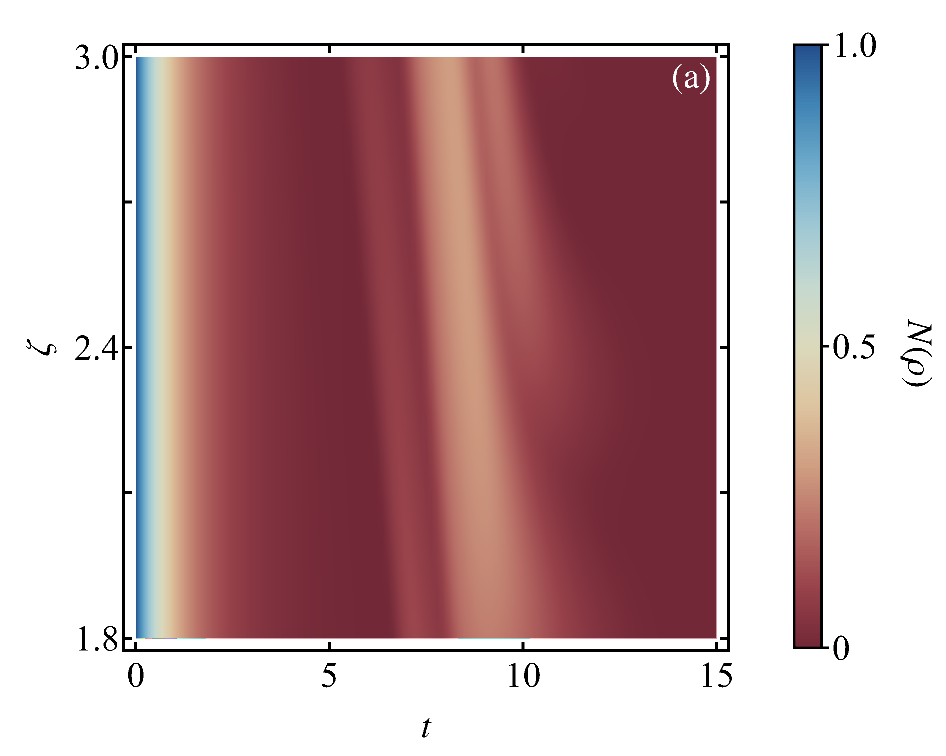
\includegraphics[width=\linewidth]{wolfram_plots/wigner_plots/densityplot_gauss4_wigner.pdf}
    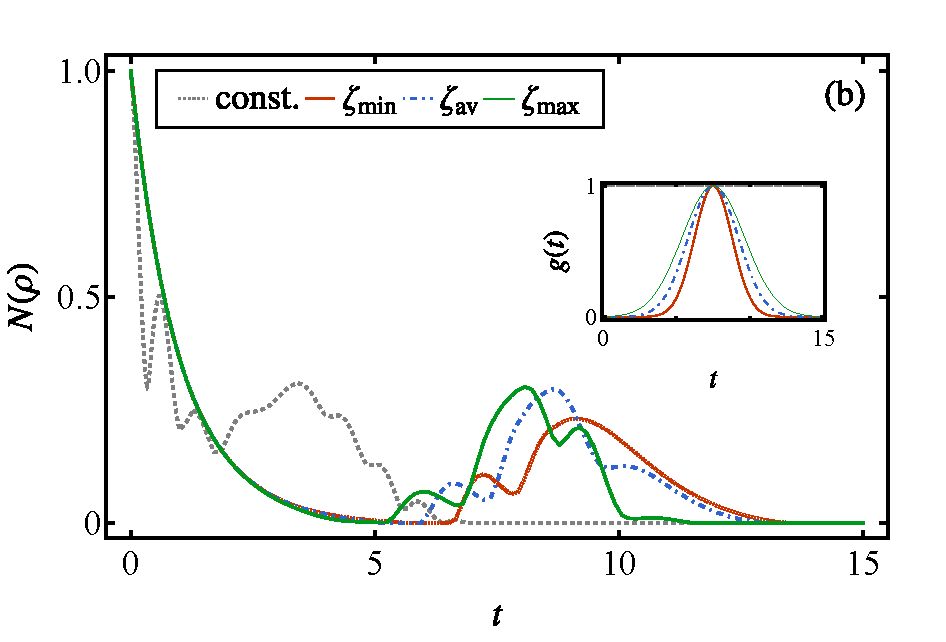
\includegraphics[width=\linewidth]{wolfram_plots/wigner_plots/plottimeev_gauss4_wigner.pdf}
    \caption{
    Behavior of the normalized Wigner negativity considering the initial state Eq. \eqref{eq:init_cat}, and the gaussian modulation for the coupling, for different widths $\zeta$ of the gaussian envelope, fixing $T=7.5$ and $\sigma=-1$.
  In (a), we consider a density plot for the time evolution of $N(\rho)$ for the range of values  $\zeta_{\text{min}} \leq \zeta \leq \zeta_{\text{max}}$, where $\zeta_{\text{min}}=1.8$ and $\zeta_{\text{max}}=3$.
   In (b), we present the time evolution for the constant coupling (dashed gray line), $\zeta_{\text{min}}$ (dotted red line),
  $\zeta_{\text{av}}=(\zeta_{\text{min}}+\zeta_{\text{max}})/2$ (dot-dashed blue line) and
  $\zeta_{\text{max}}$ (solid green line), with the time evolution of the coupling as an inset.
  }
    \label{fig:wigner_gauss4}
\end{figure}

\begin{figure}
    \centering
    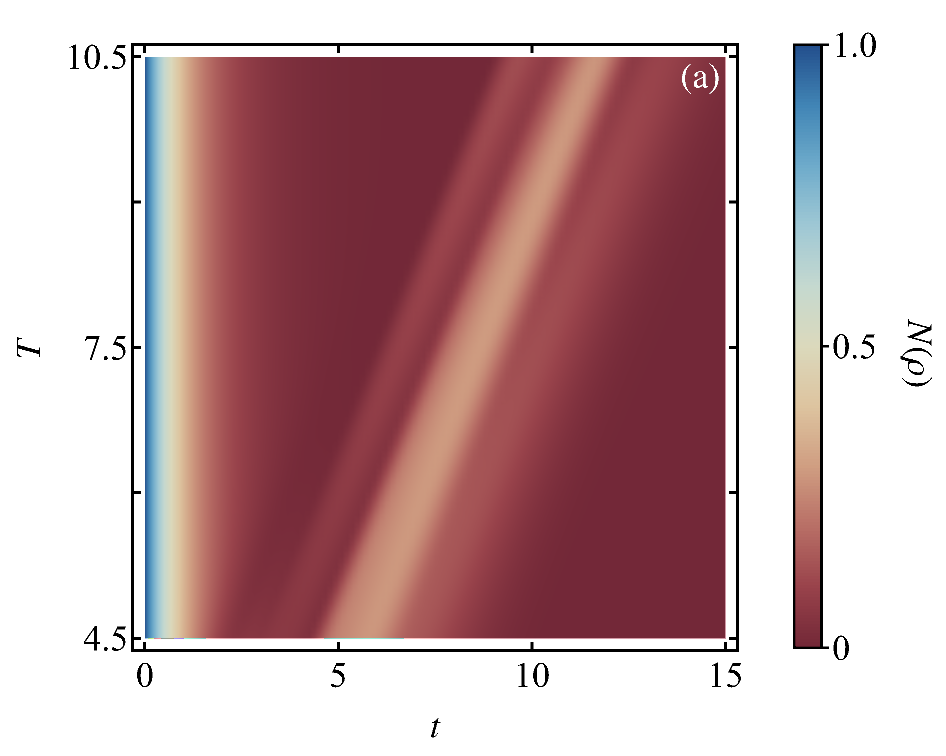
\includegraphics[width=\linewidth]{wolfram_plots/wigner_plots/densityplot_gauss6_wigner.pdf}
    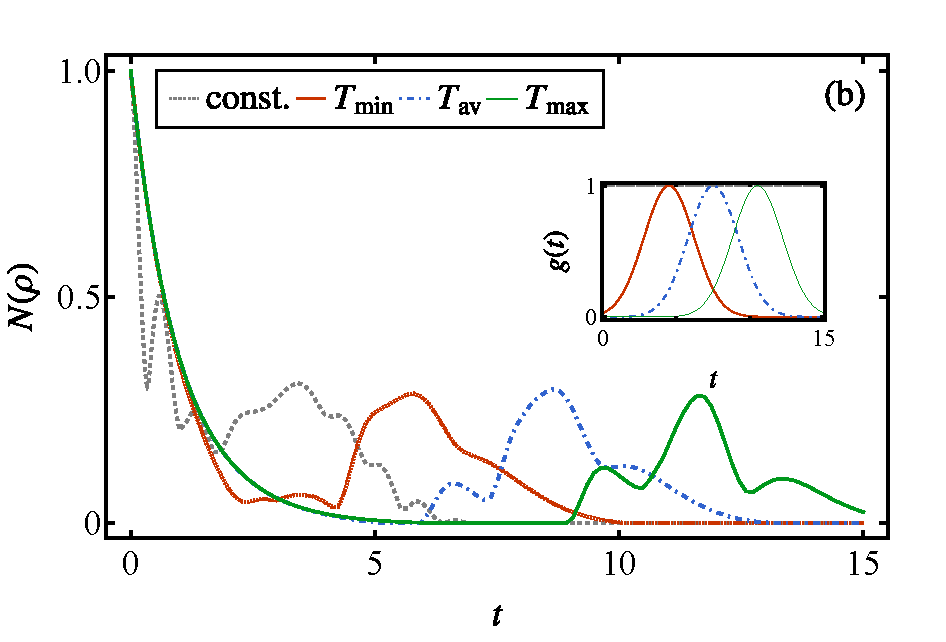
\includegraphics[width=\linewidth]{wolfram_plots/wigner_plots/plottimeev_gauss6_wigner.pdf}
    \caption{
  Behavior of the normalized Wigner negativity considering the initial state Eq. \eqref{eq:init_cat}, and the gaussian modulation for the coupling, for different instants of peak $T$ of the gaussian envelope, fixing $\zeta=2.4$ and $\sigma=-1$.
  In (a), we consider a density plot for the time evolution of $N(\rho)$ for the range of values  $T_{\text{min}}\leq T \leq T_{\text{max}}$, where $T_{\text{min}}=4.5$ and $T_{\text{max}}=10.5$.
   In (b), we present the time evolution for the constant coupling (dashed gray line), $T_{\text{min}}$ (dotted red line),
  $T_{\text{av}}=(T_{\text{min}}+T_{\text{max}})/2$ (dot-dashed blue line) and
  $T_{\text{max}}$ (solid green line), with the time evolution of the coupling as an inset.
  }
    \label{fig:wigner_gauss6}
\end{figure}

\begin{figure}
    \centering
    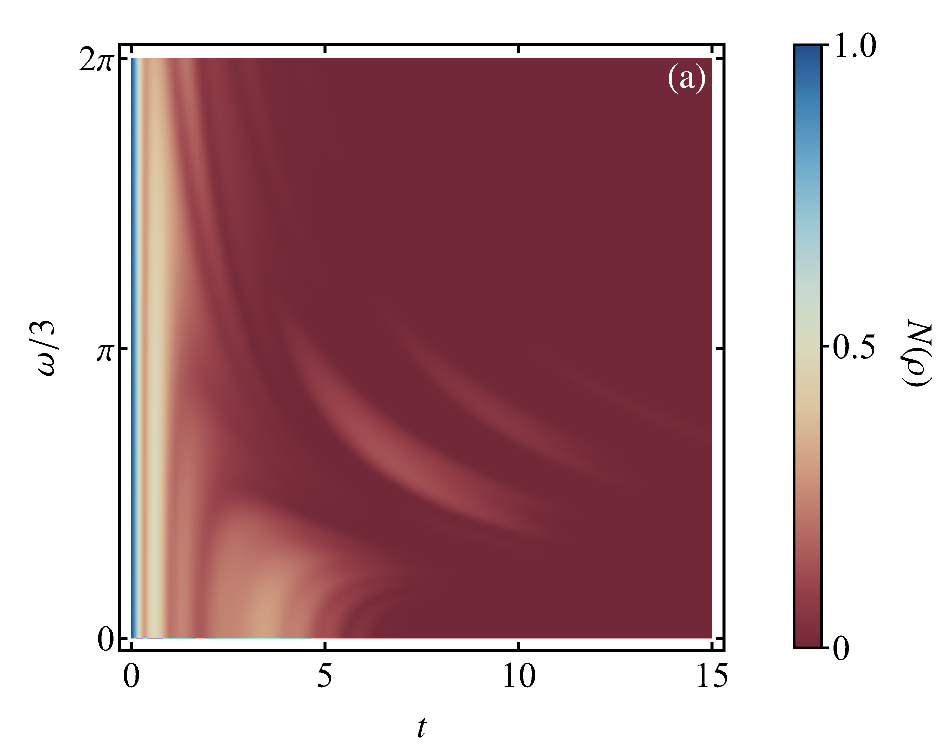
\includegraphics[width=\linewidth]{wolfram_plots/wigner_plots/densityplot_cos1_wigner.pdf}
    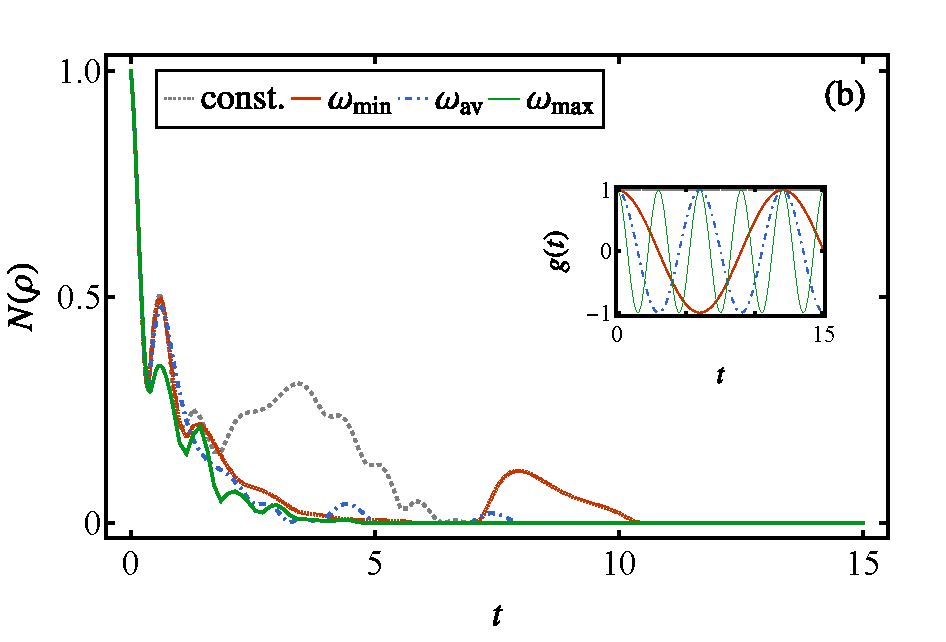
\includegraphics[width=\linewidth]{wolfram_plots/wigner_plots/plottimeev_cos1_wigner.pdf}
    \caption{
  Behavior of the normalized Wigner negativity considering the initial state Eq. \eqref{eq:init_cat}, and the cosine modulation for the coupling, for different frequencies $\omega$ and fixing $\phi=0$. 
  In (a), we consider a density plot for the time evolution of $N(\rho)$ for the range of values  $\omega_{\text{min}}\leq\omega\leq\omega_{\text{max}}$, where $\omega_{\text{min}}=\pi/6$ and $\omega_{\text{max}}=2\pi/3$.
   In (b), we present the time evolution for the constant coupling (dashed gray line), $\omega_{\text{min}}$ (dotted red line),
  $\omega_{\text{av}}=\omega_{\text{max}}/2$ (dot-dashed blue line) and
  $\omega_{\text{max}}$ (solid green line), with the time evolution of the coupling as an inset.
  }
    \label{fig:wigner_cos1}
\end{figure}

To better grasp the evolution of the Wigner negativity in the open TDJC model, 
we analyze the behavior of the Wigner function for the various coupling modulations.
Figure~\ref{fig:wigner_t000} shows the initial state Wigner function, while Fig.~\ref{fig:wigner} presents its time evolution for the various coupling profiles. Additionally, Fig.~\ref{fig:grid} displays the dynamics of the time-dependent couplings alongside the expectation values of $\hat{\sigma}_z$ and $\hat{n}$.
Interestingly, both Gaussian modulations induce a controlled enhancement of the Wigner negativity 
associated with an oscillation in the coupling. 
This oscillation can be interpreted as enabling an excitation 
transfer from the atom to the field; following this exchange, an increase in the Wigner negativity is observed. 
\emph{A priori}, one might expect that this quantum exchange would also help sustain non-classicality in the trigonometric case, 
but this is not observed. Instead, it appears that the trigonometric modulation merely causes rotations of the Wigner 
function in phase space without yielding any significant enhancement of its negativity.

\begin{figure}
    \centering
    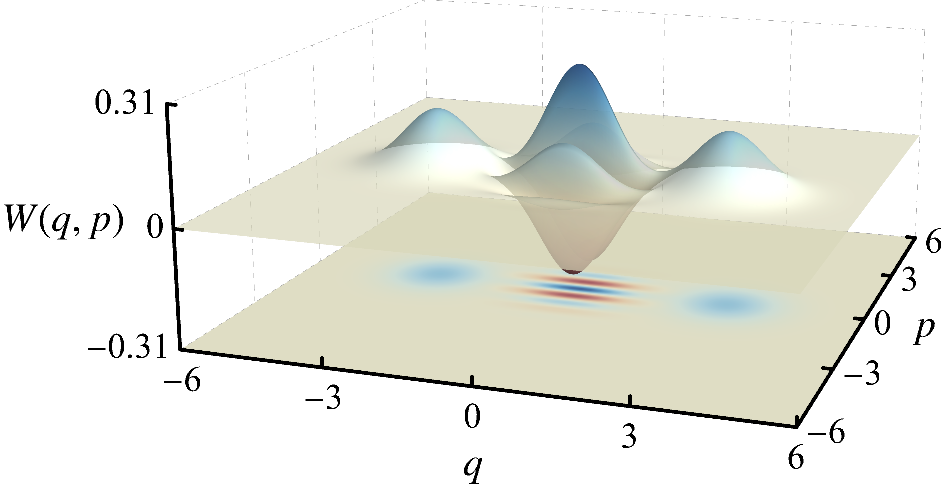
\includegraphics[width=\linewidth]{wolfram_plots/wigner_plots/const_t000.pdf}
    \caption{
Time-evolution of the Wigner function for the initial state in 
Eq.~\eqref{eq:init_cat}. 
  }
    \label{fig:wigner_t000}
\end{figure}


\begin{figure*}
    \centering
    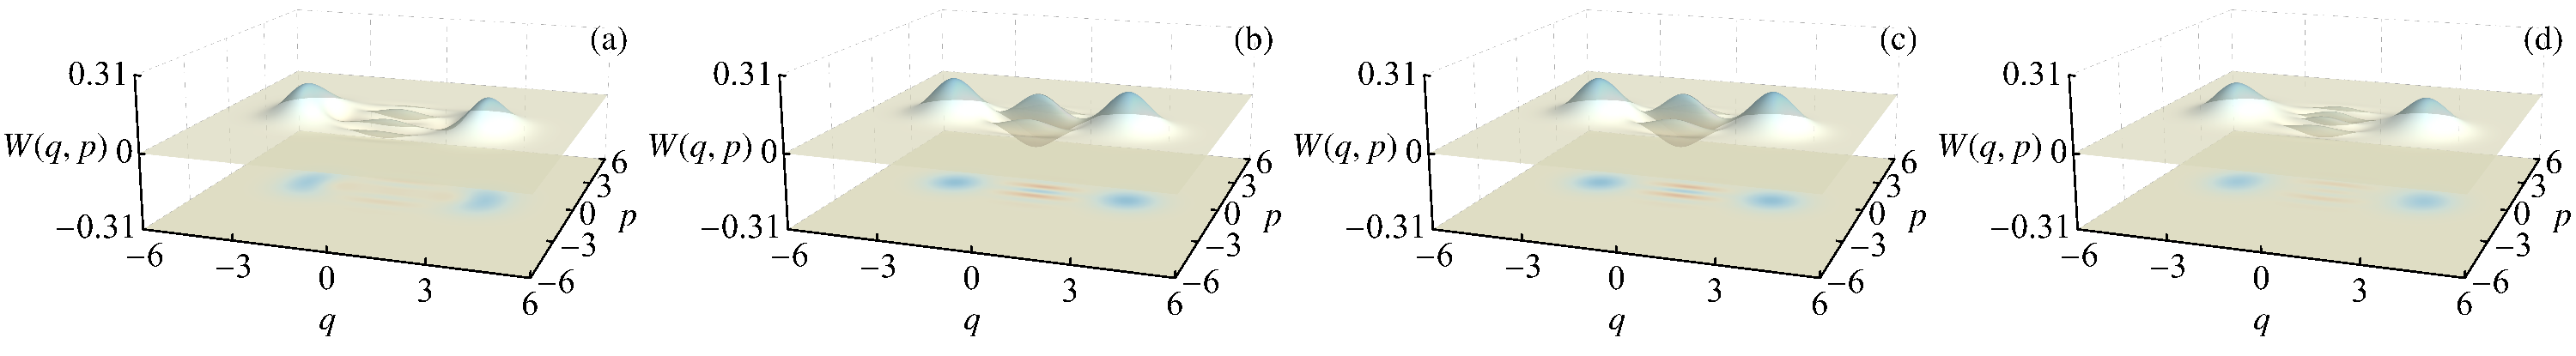
\includegraphics[width=\linewidth]{wolfram_plots/wigner_plots/timeframes_wigner_firstrow.pdf}
     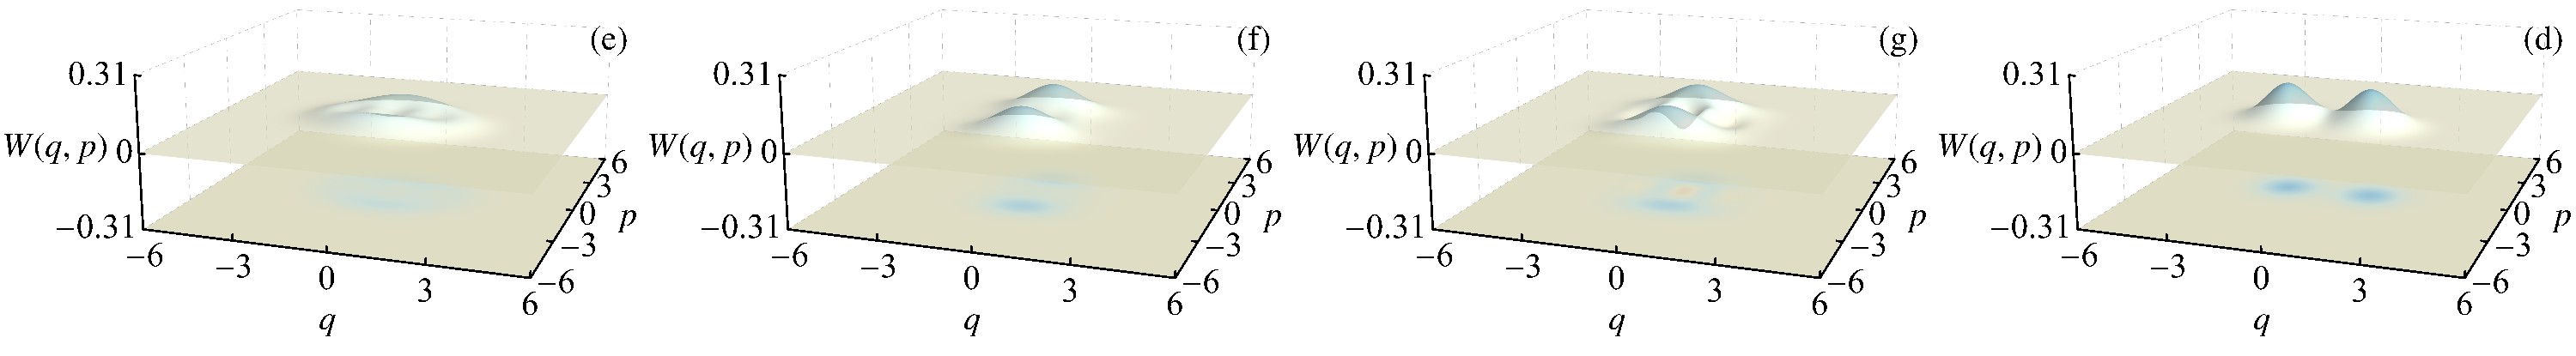
\includegraphics[width=\linewidth]{wolfram_plots/wigner_plots/timeframes_wigner_secondrow.pdf}
    \caption{
Time-evolution of the Wigner function for the initial state in Eq.~\eqref{eq:init_cat}. 
The columns from left to right show the Wigner function for the four different coupling profiles: 
constant coupling (a, e), Gaussian with varying width (b, f), Gaussian with peak time change (c, g), 
and cosine profile (d, h). 
The first row corresponds to an intermediate time $t=7.5$ (a, b, c, d), 
while the second row shows the final time $t=15$ (e, f, g, h). 
The parameters for each profile are: 
constant coupling ($g_0=1$); 
Gaussian with varying width ($g_0=1, \sigma=-1, \zeta_\text{max}=3, T=7.5$); 
Gaussian with peak time change ($g_0=1, \sigma=-1, \zeta=2.4, T_\text{max}=10.5$); 
and cosine profile ($g_0=1, \phi=0, \omega_\text{max}=2\pi/3$).
  }
    \label{fig:wigner}
\end{figure*}

\begin{figure*}
    \centering
    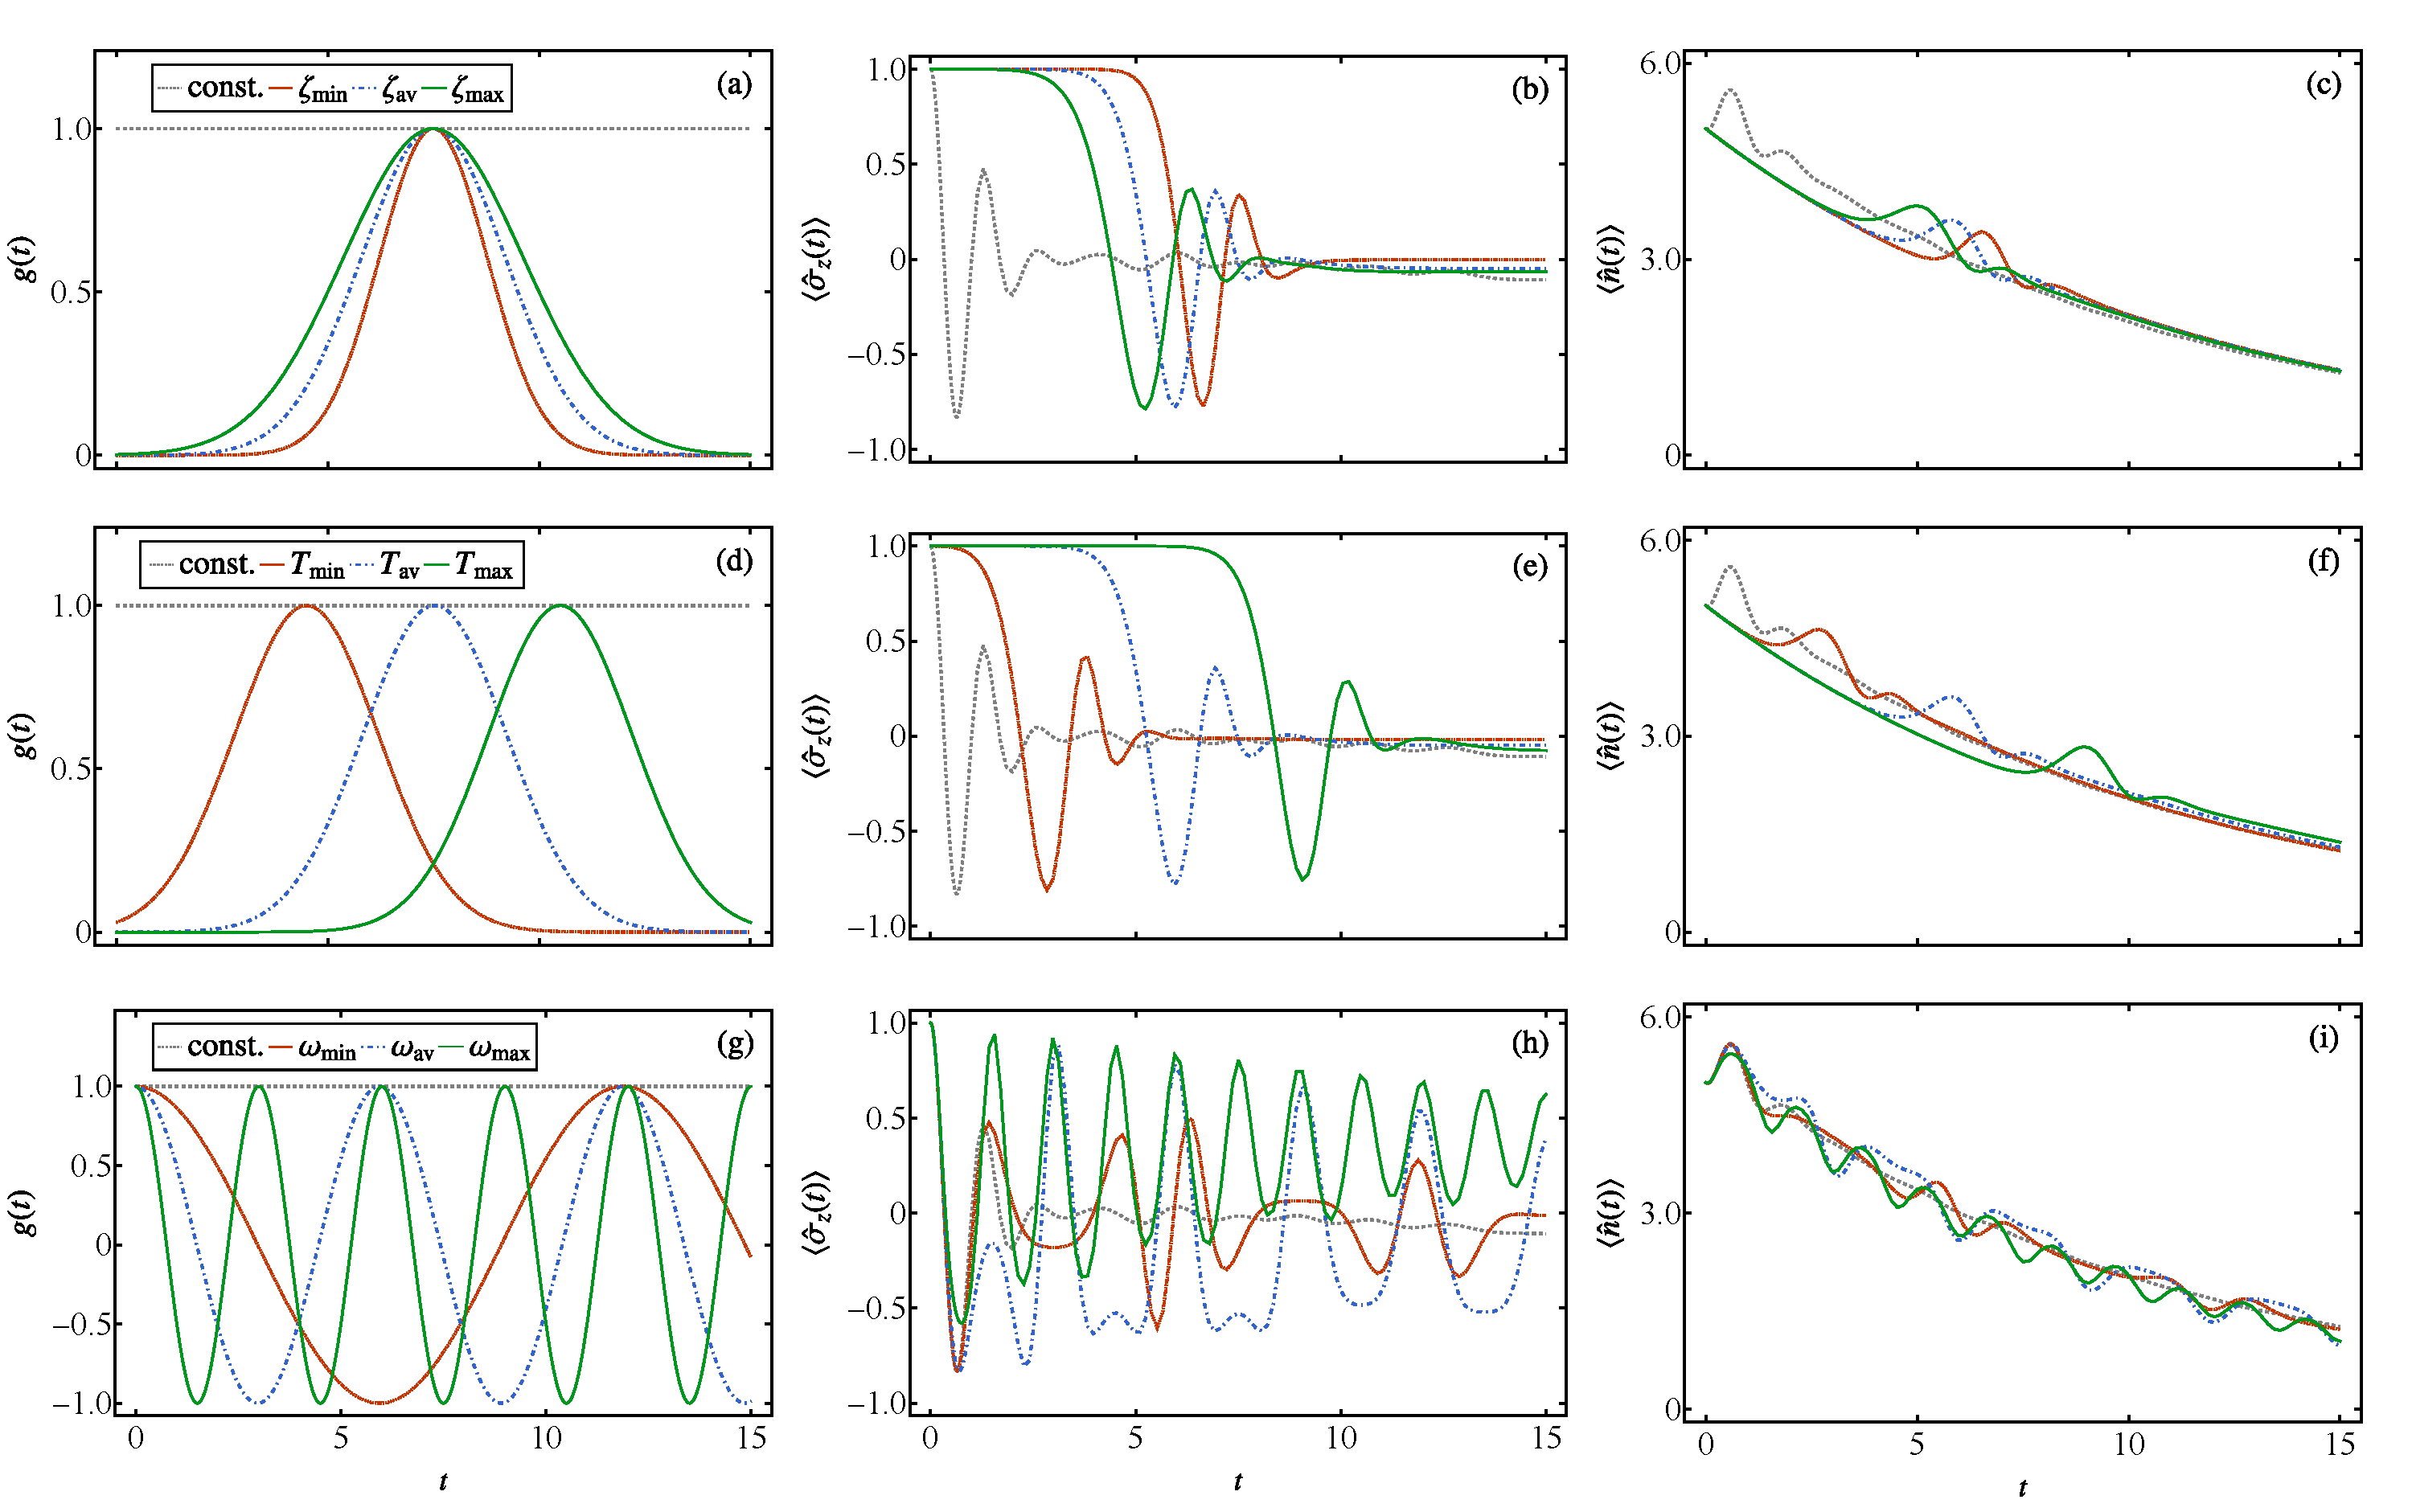
\includegraphics[width=\linewidth]{wolfram_plots/grid}
    \caption{
Time-evolution of the couplings and the expectation values of the operators 
$\hat{\sigma}_z$ and $\hat{n}$ for the initial state in Eq. \eqref{eq:init_cat}. 
Panels (a), (d), and (g) display the time-dependent couplings, featuring 
Gaussian pulses with varying widths in (a), adjusted peak times in (d), and a cosine profile in (g). 
The remaining panels show the corresponding 
expectation values for the observables $\hat{\sigma}_z$ and $\hat{n}$, 
organized by rows that match each specific modulation parameter set.
Panels (b) and (c) (first row) use the same 
parameters as Fig.~\ref{fig:wigner_gauss4}; panels (e) and (f) (second row) 
correspond to Fig.~\ref{fig:wigner_gauss6}; and panels (h) and (i) (third row) 
correspond to Fig.~\ref{fig:wigner_cos1}. 
Within these rows, the results for 
$\hat{\sigma}_z$ are plotted in (b), (e), and (h), while those for $\hat{n}$ 
are displayed in (c), (f), and (i).
  }
    \label{fig:grid}
\end{figure*}

\subsection{Coherence}
\label{subsec: coherence}
Coherence refers to the ability of a quantum state to maintain a superposition of the eigenstates of a given observable. 
Considering a two-level system (qubit) in the basis of $\hat{\sigma}_z$, denoted by $\{|e\rangle,|g\rangle\}$, any density matrix with a nonzero off-diagonal element possesses a certain amount of coherence \cite{Messinger2019,Streltsov2017}.
To quantify the coherence in the qubit, we use the relative entropy of coherence \cite{Baumgratz2014}, given by,
\begin{equation}
    C(\rho^{Q}) = S(\rho^{Q}_{\text{diag}}) - S(\rho^{Q}),
    \label{eq:coherence_qubit}
\end{equation}
where $S(\cdot)$ is the von Neumann entropy \cite{VonNeumann1927b,Nielsen2010}, $\rho^{Q}=\text{tr}_F(\rho)=\sum_n \langle n|\rho|n\rangle$ is the reduced qubit state and 
\begin{equation}
    \rho^{Q}_{\text{diag}}=\sum_{i=e,g}|i\rangle \langle i|\rho^{Q}|i\rangle \langle i|.
\end{equation} 
The quantifier satisfies $C(\rho^{Q}) \leq S(\rho^{Q}_{\text{diag}}) \leq \log(d)$,
where $d$ is the dimension of the basis.
For the von Neumann entropy in Eq. \eqref{eq:coherence_qubit}, we take the logarithm in base $2$, which ensures normalization for the two-level system $(d=2)$.

For the analysis presented in this section, the qubit is initialized in a maximally coherent superposition, i.e. the eigenstate $|+\rangle$ of $\hat{\sigma}_x$,
while the field starts in a coherent state $|\alpha\rangle = \sum_{n} e^{-|\alpha|^2/2} \alpha^n/\sqrt{n!} |n\rangle$ \cite{Glauber1963c,GERRY2005}.
Both the atomic and cavity initial states are accessible in CQED experiments \cite{Brune1996,Marrocco2005,Haroche2013}. 
The initial global state of the system is
\begin{equation} \label{eq:superposition}
|\psi(0)\rangle = \frac{1}{\sqrt{2}} \left( |e\rangle + |g\rangle \right) |\alpha\rangle.
\end{equation}
In Ref. \cite{Mortezapour2017b}, the $l_1$-norm of coherence of a moving qubit inside a leaky cavity was studied, but with the cavity initially in the vacuum state and a different treatment of cavity dissipation.

We first consider the atomic coherence under Gaussian coupling, as given by Eq. \eqref{eq:coherence_qubit}.
In Fig. \ref{fig:coer_gauss4}, we analyze the effects of varying the width $\zeta$ of the Gaussian envelope, with fixed parameters $T = 25$ and $\sigma = -1$.
The constant coupling case (dashed gray line in Fig. \ref{fig:coer_gauss4}(b)) exhibits an overall decay. In contrast, the time-dependent cases show a certain advantage after the initial moments. This occurs because we are dealing exclusively with atomic non-classicality, and the interaction with the cavity can be seen as an additional source of damping for certain coupling values \cite{Auffeves2010}.
Thus, the time-dependent cases, with their initially small coupling, gain an advantage by suppressing this additional loss channel at the outset, thereby preserving $C_{\text{max}}(\rho^{Q})$.
In this context, as shown in Fig. \ref{fig:coer_gauss4}(a), at later times a narrower Gaussian envelope leads to higher coherence, whereas a broader envelope results in lower coherence.
The effect of shifting the coupling's peak time, shown in Fig. \ref{fig:coer_gauss6} for fixed $\zeta=8$ and $\sigma=-1$, also yields an advantage over the constant coupling case, with a slightly better outcome for the delayed peak.

Therefore, this form of coupling may significantly enhance the generation and persistence of atomic coherence. 
In particular, both varying the width of the Gaussian envelope and shifting the position of its center lead to a considerable increase in the non-classicality achieved during the dynamics. 

The cases presented above start from $g(0)=0$, which benefits the maintenance of an atomic-only non-classicality.
This behavior might suggest that advantages of using a time-dependent coupling over a constant coupling only arise in such situations. 
However, in Fig.~\ref{fig:coer_cos5} we present the results for the coupling given by Eq.~\eqref{eq:sin_coup}, with $\phi = 0$ and $6 < \omega < 10$. 
The oscillatory nature of the coupling induces a corresponding oscillatory behavior in the non-classicality, which in turn delays its decay.

\ca{Estou tentando mudar o menos possível os parametros. Por isso, para todoas as simulações estou utilizando $\alpha=\sqrt{5}$. Posso ver outros valores, mas foi o melhor que consegui para fazer na Wigner. Uma outra possibilidade é usar estados de fock para Wigner.}

\begin{figure}
    \centering
    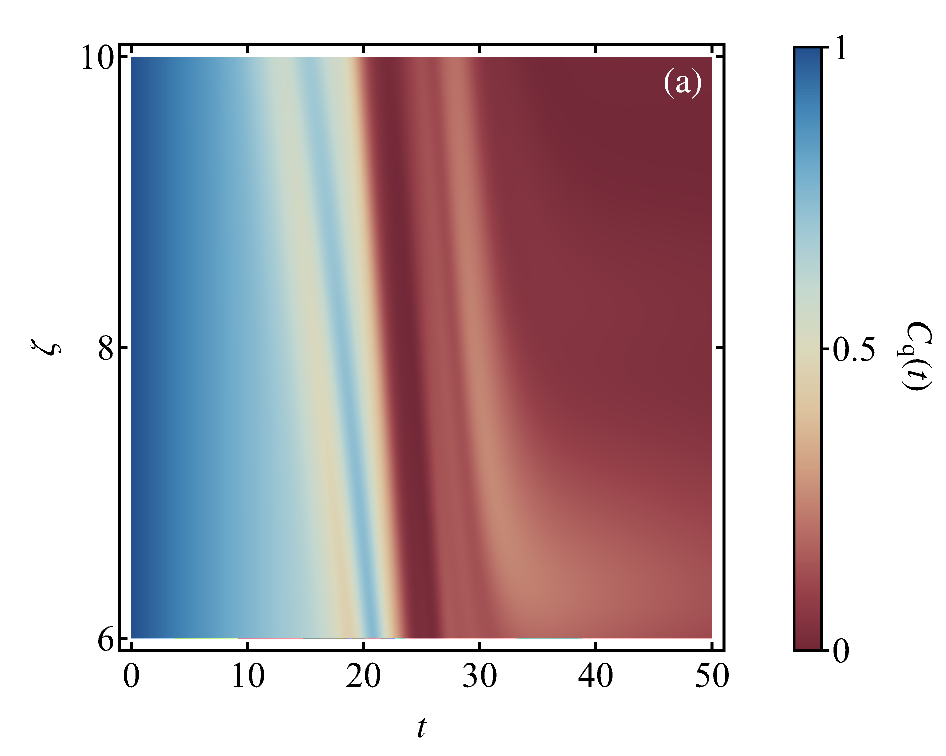
\includegraphics[width=\linewidth]{wolfram_plots/coerence_plots/densityplotcombinedcoer_gauss4.pdf}
    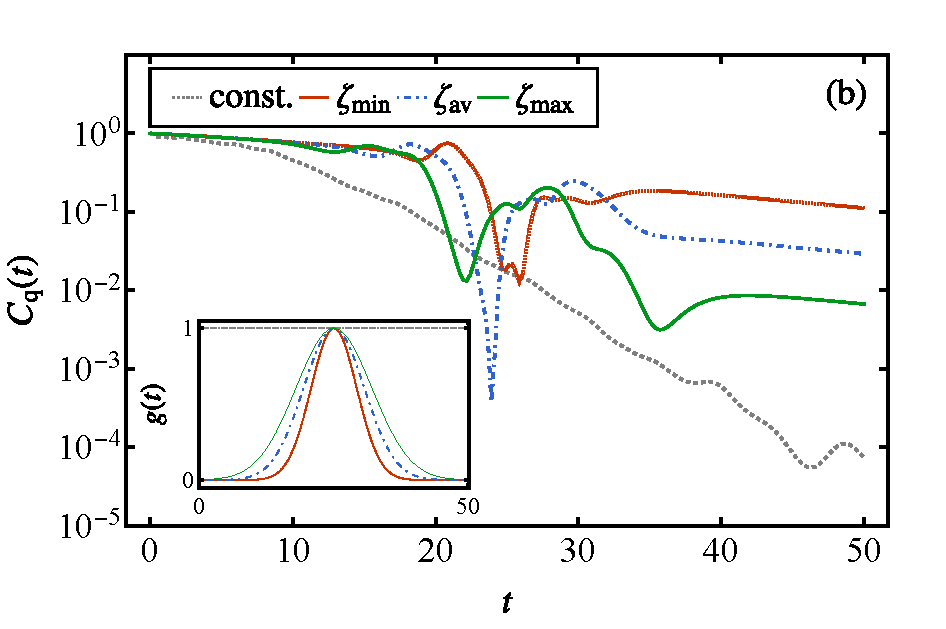
\includegraphics[width=\linewidth]{wolfram_plots/coerence_plots/plottimeev_gauss4.pdf}
    \caption{
  Behavior of the atomic coherence considering the initial state Eq. \eqref{eq:superposition}, and the gaussian modulation for the coupling, for different widths $\zeta$ of the gaussian envelope, fixing $T=25$ and $\sigma=-1$.
  In (a), we consider a density plot for the time evolution of $C_\text{q}(t)$ for the range of values  $\zeta_{\text{min}} \leq \zeta \leq \zeta_{\text{max}}$, where $\zeta_{\text{min}}=6$ and $\zeta_{\text{max}}=10$.
   In (b), we present the time evolution of the coherence on a logarithmic scale for four cases: constant coupling (dashed gray line), $\zeta_{\text{min}}$ (dotted red line), the average value $\zeta_{\text{av}} = (\zeta_{\text{min}} + \zeta_{\text{max}})/2$ (dot-dashed blue line), and $\zeta_{\text{max}}$ (solid green line).
The time evolution of the coupling itself is shown in the inset (plotted on a standard scale).
\ts{O caso average desse deveria bater com o caso average da figura anterior. Acho que não está batendo por causa daquela diferença nos pontos médios.}
\ts{Colocar uma linha magenta no valor fixado como lower bound.}
  }
    \label{fig:coer_gauss4}
\end{figure}

\begin{figure}
    \centering
    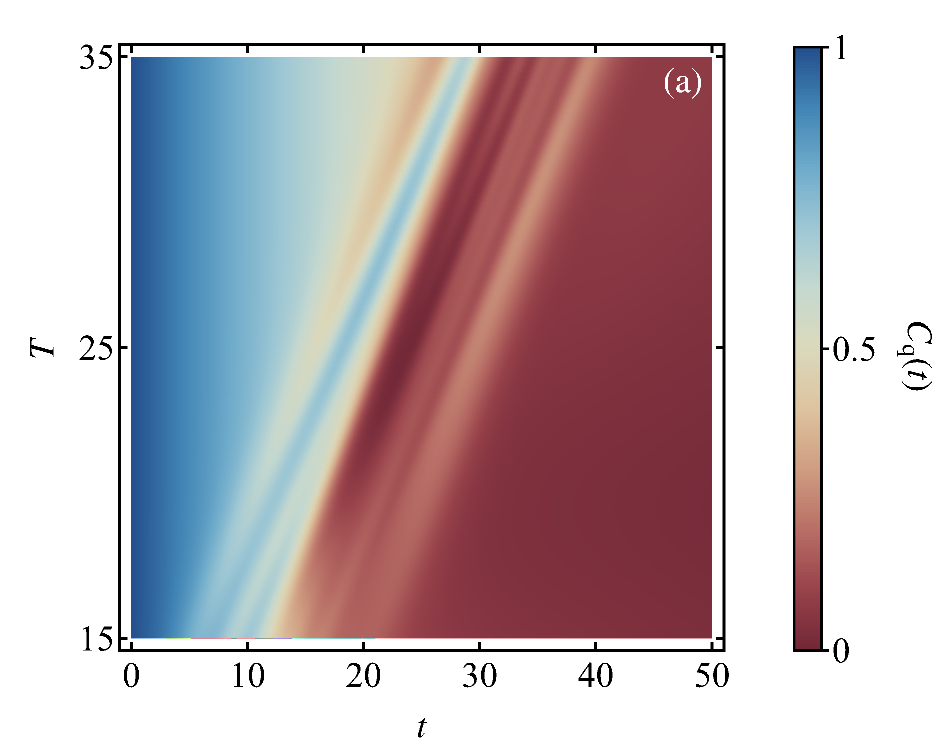
\includegraphics[width=\linewidth]{wolfram_plots/coerence_plots/densityplotcombinedcoer_gauss6.pdf}
    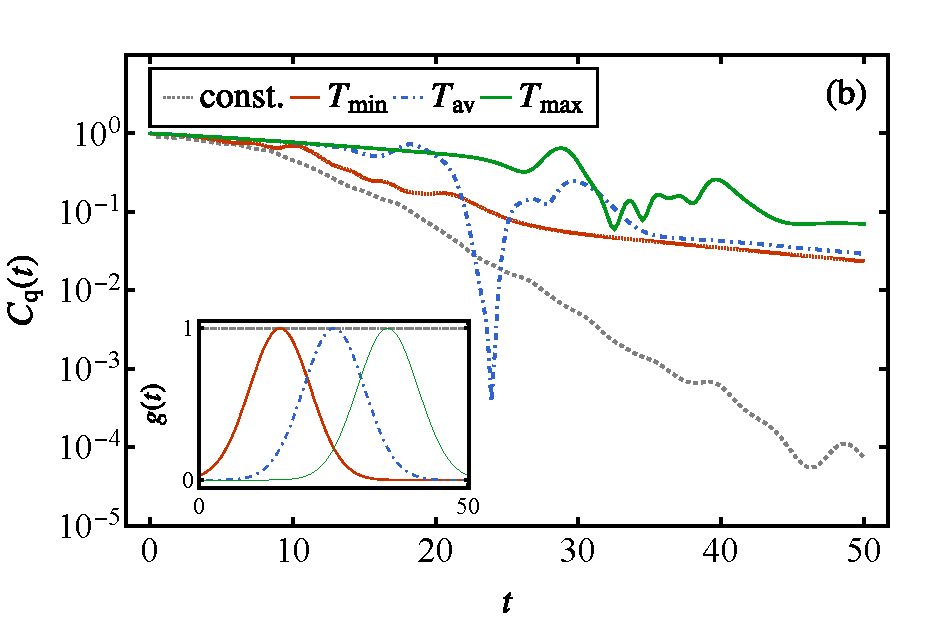
\includegraphics[width=\linewidth]{wolfram_plots/coerence_plots/plottimeev_gauss6.pdf}
    \caption{
  Behavior of the atomic coherence considering the initial state Eq. \eqref{eq:superposition}, and the gaussian modulation for the coupling, for different instants of peak $T$ of the gaussian envelope, fixing $\zeta=8$ and $\sigma=-1$.
  In (a), we consider a density plot for the time evolution of $C_\text{q}(t)$ for the range of values  $T_{\text{min}}\leq T \leq T_{\text{max}}$, where $T_{\text{min}}=15$ and $T_{\text{max}}=35$.
In (b), we present the time evolution of the coherence on a logarithmic scale for four cases: constant coupling (dashed gray line), $T_{\text{min}}$ (dotted red line),
  $T_{\text{av}}=(T_{\text{min}}+T_{\text{max}})/2$ (dot-dashed blue line) and
  $T_{\text{max}}$ (solid green line).
The time evolution of the coupling itself is shown in the inset (plotted on a standard scale).
  }
    \label{fig:coer_gauss6}
\end{figure}

\begin{figure}
    \centering
    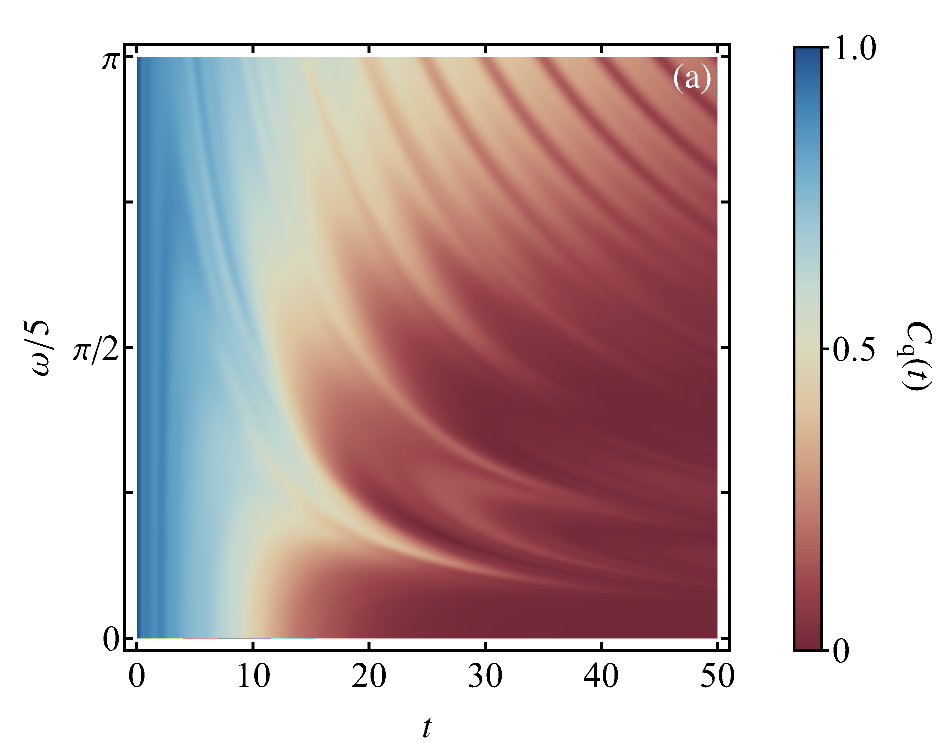
\includegraphics[width=\linewidth]{wolfram_plots/coerence_plots/densityplot_cos5_coer.pdf}
    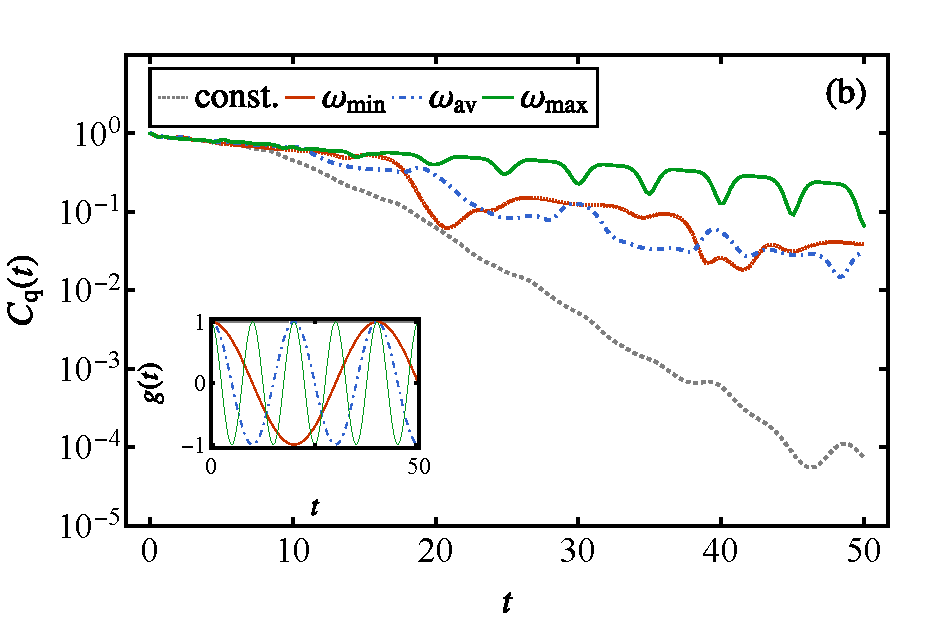
\includegraphics[width=\linewidth]{wolfram_plots/coerence_plots/plottimeev_cos5_coer.pdf}
    \caption{
 Behavior of the atomic coherence considering the initial state Eq. \eqref{eq:superposition}, and the cosine modulation for the coupling, for different frequencies $\omega$ and fixing $\phi=0$. 
  In (a), we consider a density plot for the time evolution of $C_\text{q}(t)$ for the range of values  $\omega_{\text{min}}\leq\omega\leq\omega_{\text{max}}$, where $\omega_{\text{min}}=\pi/20$ and $\omega_{\text{max}}=\pi/5$.
   In (b), we present the time evolution of the coherence on a logarithmic scale for four cases: constant coupling (dashed gray line), $\omega_{\text{min}}$ (dotted red line),
  $\omega_{\text{av}}=\omega_{\text{max}}/2$ (dot-dashed blue line) and
  $\omega_{\text{max}}$ (solid green line).
  The time evolution of the coupling itself is shown in the inset (plotted on a standard scale).
  }
    \label{fig:coer_cos5}
\end{figure}


%\begin{figure}
%    \centering
%    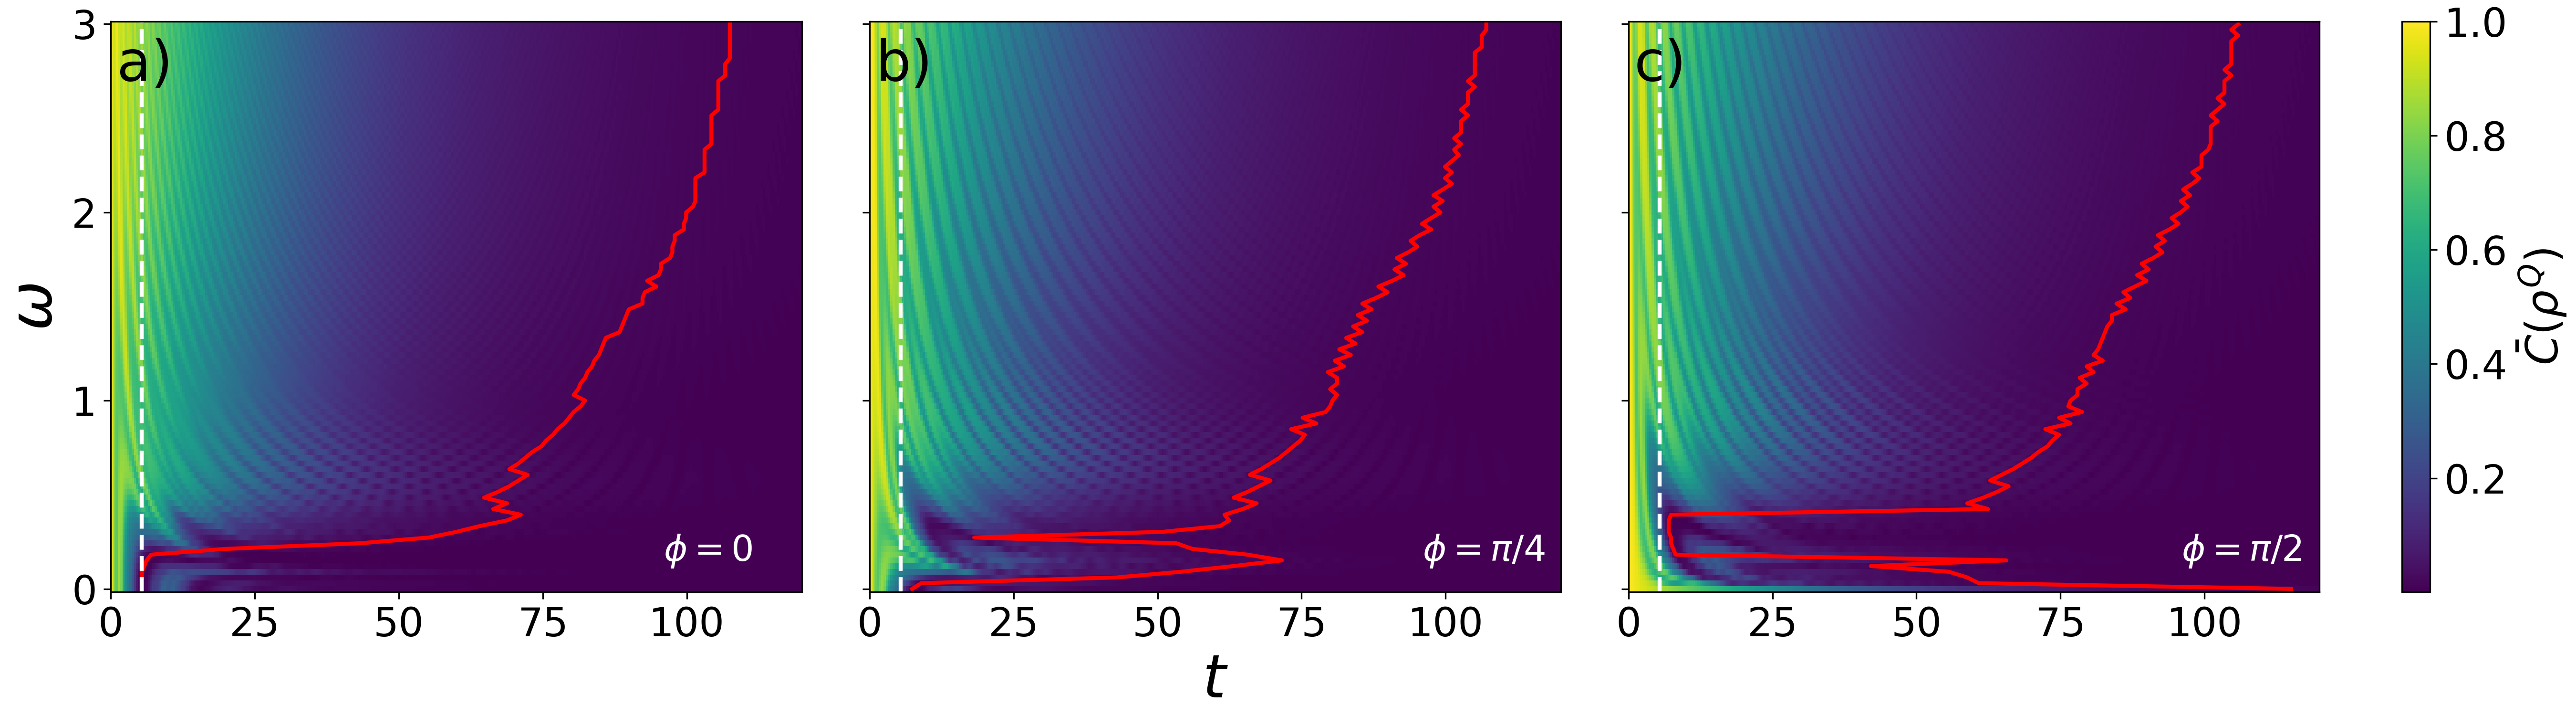
\includegraphics[width=\linewidth]{paper_images/coerence.png}
%    \caption{Caption}
%    \label{fig:placeholder}
%\end{figure}

%\begin{figure}
%    \centering
%    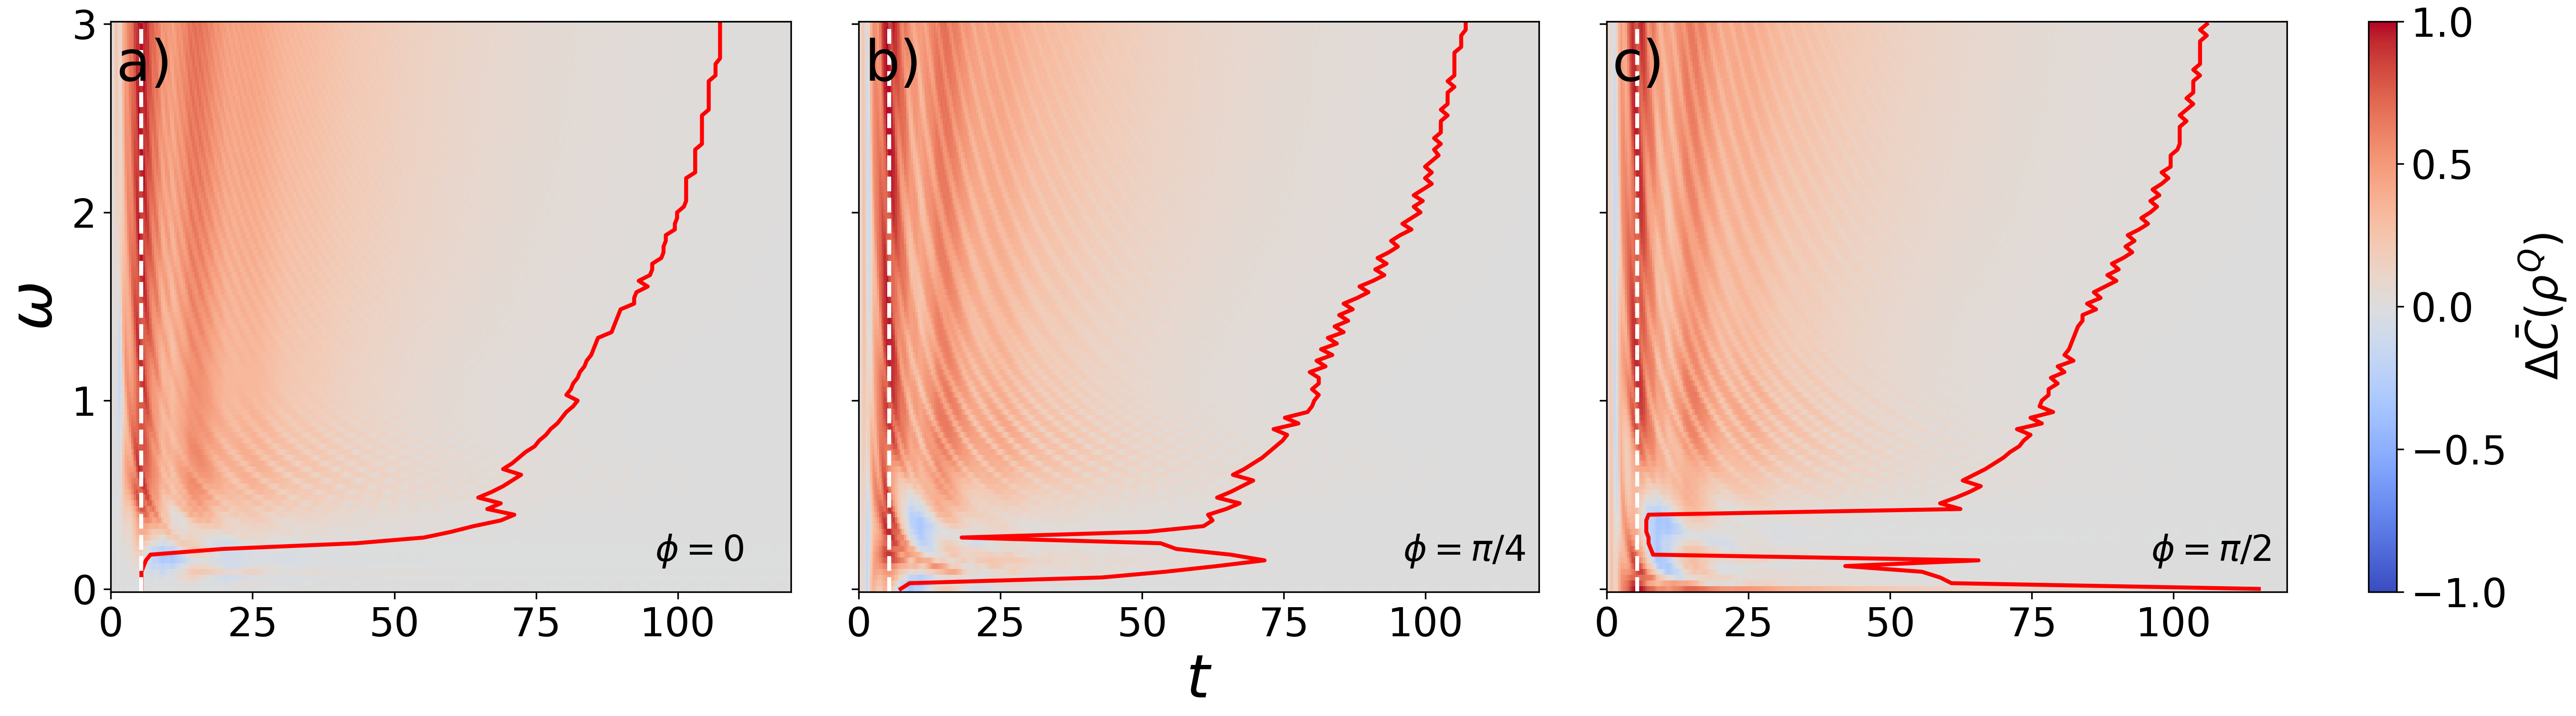
\includegraphics[width=\linewidth]{paper_images/coerence_delta.png}
%    \caption{Caption}
%    \label{fig:placeholder}
%\end{figure}

\subsection{Quantum Magic}
\label{subsec:magic}
Quantum magic is a property of the state that characterizes its nonstabilizerness \cite{Bravyi2005,Mittal2026}.
In the context of quantum resource theories, magic states allow the implementation of gates that cannot be efficiently simulated in classical computers \cite{Chitambar2019}.

Here, we study the magic of the atom (qubit). 
The dynamics of atomic magic have been studied for the JC model in Ref. \cite{Shuangshuang2023}, analyzing how the magic can build up from stabilizer states in the dynamics of the model in a closed-system scenario. 

As a quantifier of quantum magic, we employ the stabilizer $\alpha$-Réniy entropy  \cite{Leone2022,Brokemeier2025,Mittal2026} $M_\alpha(\rho)$, which can be measured experimentally via Pauli tomography \cite{Oliviero2022}.
We employ $\alpha=2$,  with $M_\alpha(\rho)$ obeying
\begin{equation}
M_2(\rho) =-\log \left( \frac{\sum_{\hat{P} \in \mathcal{P}} |\mathrm{Tr}(\rho \hat{P})|^{4}}{\sum_{\hat{P} \in \mathcal{P}} |\mathrm{Tr}(\rho \hat{P}) |^2} \right),
\end{equation}
%\begin{equation}
%M_\alpha(\rho) = \frac{1}{1-\alpha} \log \left( %\frac{\sum_{P \in \mathcal{P}} |\mathrm{Tr}(\rho %P)|^{2\alpha}}{\sum_{P \in \mathcal{P}} |\mathrm{Tr}(\rho %P) |^2} \right)
%\end{equation}
where $\mathcal{P}=\{\mathbbm{1},\hat{\sigma}_y,\hat{\sigma}_x,\hat{\sigma}_z \}$ is the Pauli group.
Considering the case in question the quantifier is bounded by $M_2(\rho)\leq \log(3/2)\approx0.4055$ \cite{Wang2023}.

In our work, we consider an initial state of the atomic subsystem that possesses maximum magic \cite{Bravyi2005,Haug2026}, 
\begin{equation} \label{eq:max_magic}
\ket{\psi(0)} = \left(\cos\frac{\theta}{2}\ket{g} + e^{i\pi/4}\sin\frac{\theta}{2}\ket{e}\right)|\alpha \rangle,
\end{equation}
where $\cos\theta = 1/\sqrt{3}$.

In the context of quantum magic, this resource exhibits a non-trivial relationship with dissipation \cite{Oliviero2022,Mittal2026}. 
Instead of vanishing asymptotically, it reaches a steady state within certain parameter regimes. 
Under constant coupling, the magic initially decays, subsequently reemerges, and undergoes a final decay during the late-time dynamics investigated.
For a gaussian modulation with a variable envelope width (Fig. \ref{fig:magic_gauss1}), the interaction is detrimental to quantum magic, inducing oscillations before settling at an intermediate value after the interaction ceases. When varying the peak time of the Gaussian envelope (Fig. \ref{fig:magic_gauss2}), the modulation shifts the specific time interval in which these oscillations occur. Finally, in the case of trigonometric modulation (Fig. \ref{fig:magic_cos1}), higher-frequency oscillations result in better overall preservation of the state's nonstabilizerness.

\begin{figure}[!h]
    \centering
    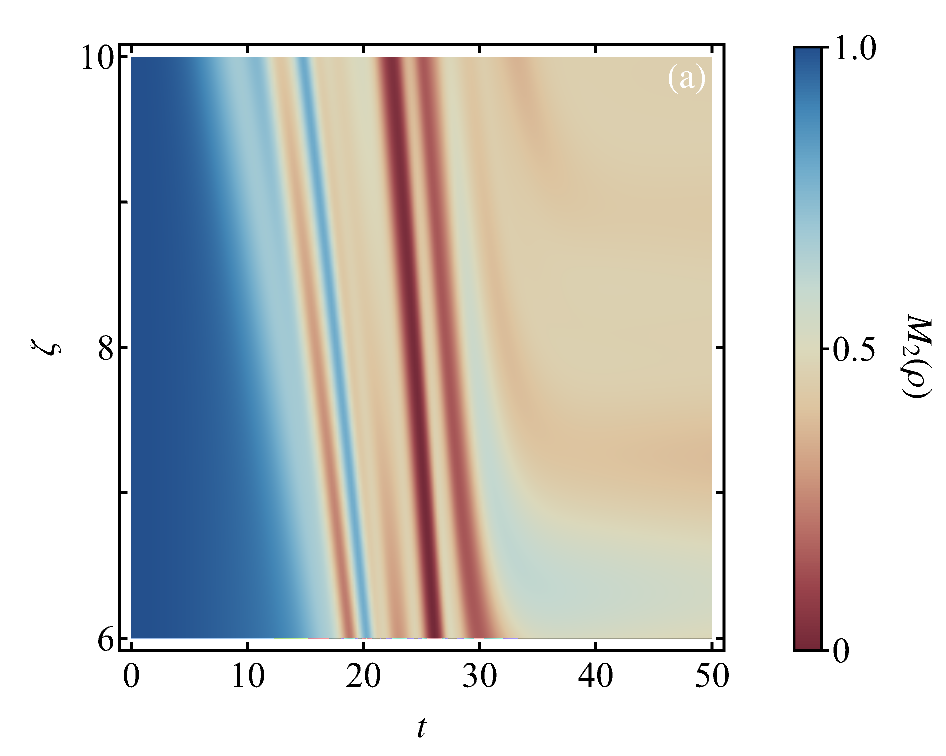
\includegraphics[width=\linewidth]{wolfram_plots/magic_plots/densityplot_gauss1_magic.pdf}
    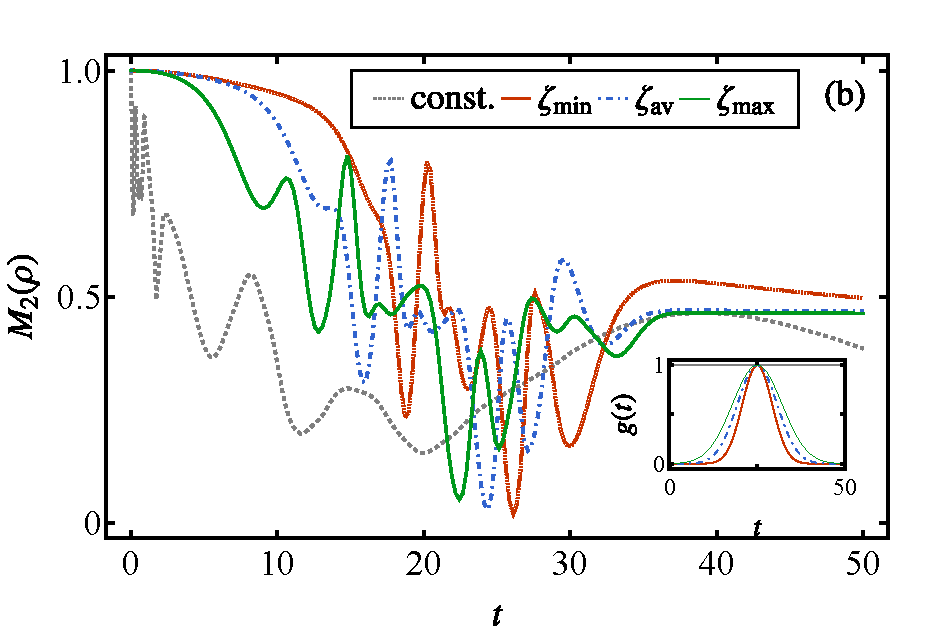
\includegraphics[width=\linewidth]{wolfram_plots/magic_plots/plottimeev_gauss1_magic.pdf}
    \caption{
    Behavior of the normalized stabilizer $2$-Réniy entropy, considering the initial state Eq. \eqref{eq:max_magic}, and the gaussian modulation for the coupling, for different widths $\zeta$ of the gaussian envelope, fixing $T=25$ and $\sigma=-1$.
  In (a), we consider a density plot for the time evolution of $N(\rho)$ for the range of values  $\zeta_{\text{min}} \leq \zeta \leq \zeta_{\text{max}}$, where $\zeta_{\text{min}}=6$ and $\zeta_{\text{max}}=10$.
   In (b), we present the time evolution for the constant coupling (dashed gray line), $\zeta_{\text{min}}$ (dotted red line),
  $\zeta_{\text{av}}=(\zeta_{\text{min}}+\zeta_{\text{max}})/2$ (dot-dashed blue line) and
  $\zeta_{\text{max}}$ (solid green line), with the time evolution of the coupling as an inset.
  }
    \label{fig:magic_gauss1}
\end{figure}

\begin{figure}
    \centering
    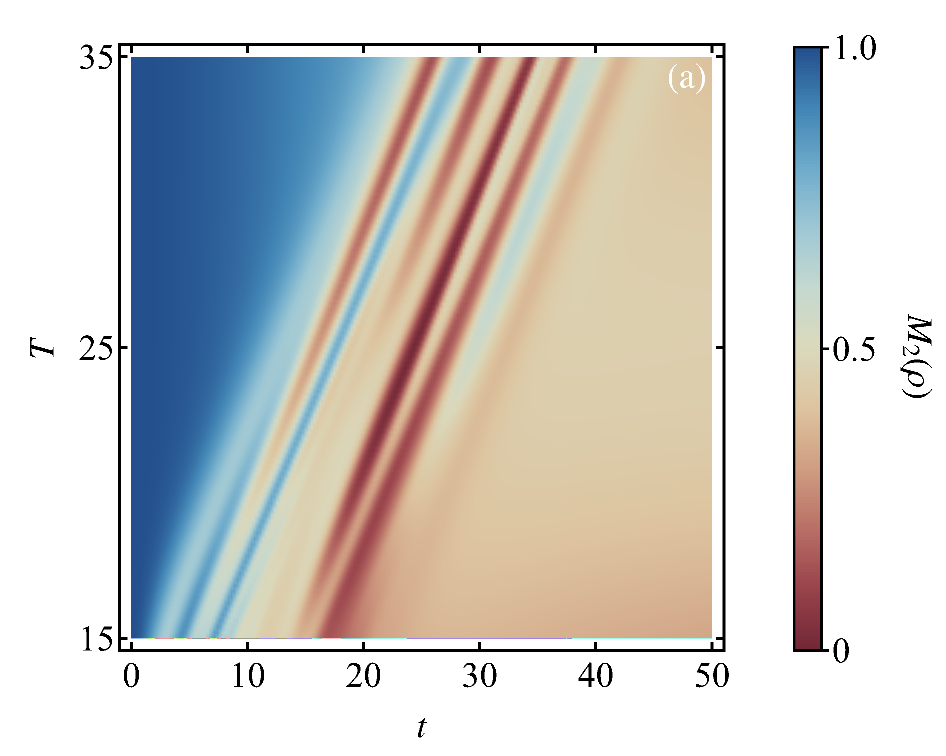
\includegraphics[width=\linewidth]{wolfram_plots/magic_plots/densityplot_gauss2_magic.pdf}
    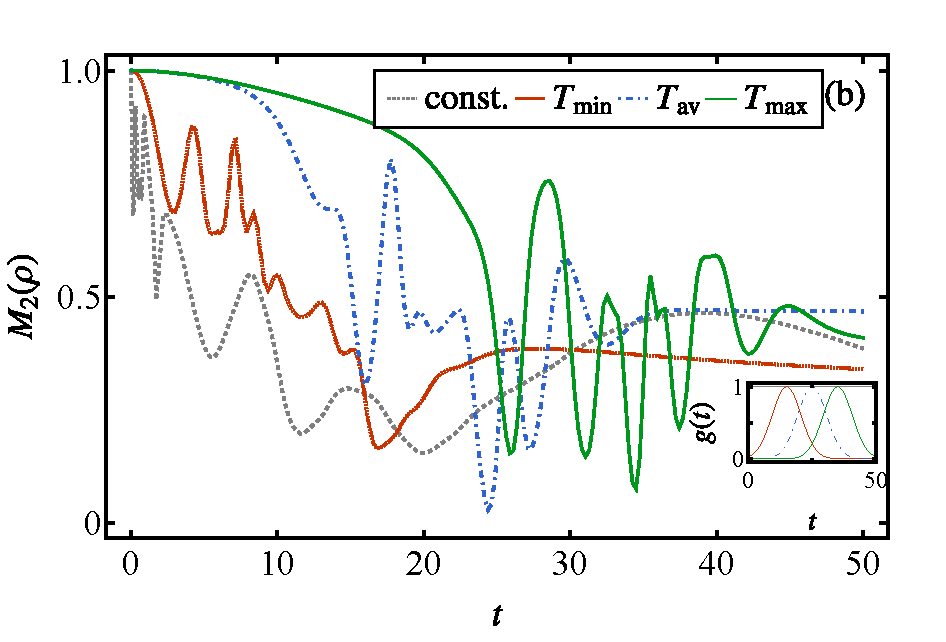
\includegraphics[width=\linewidth]{wolfram_plots/magic_plots/plottimeev_gauss2_magic.pdf}
    \caption{
  Behavior of the normalized $2$-Réniy entropy considering the initial state Eq. \eqref{eq:max_magic}, and the gaussian modulation for the coupling, for different instants of peak $T$ of the gaussian envelope, fixing $\zeta=8$ and $\sigma=-1$.
  In (a), we consider a density plot for the time evolution of $N(\rho)$ for the range of values  $T_{\text{min}}\leq T \leq T_{\text{max}}$, where $T_{\text{min}}=15$ and $T_{\text{max}}=35$.
   In (b), we present the time evolution for the constant coupling (dashed gray line), $T_{\text{min}}$ (dotted red line),
  $T_{\text{av}}=(T_{\text{min}}+T_{\text{max}})/2$ (dot-dashed blue line) and
  $T_{\text{max}}$ (solid green line), with the time evolution of the coupling as an inset.
  }
    \label{fig:magic_gauss2}
\end{figure}

\begin{figure}
    \centering
    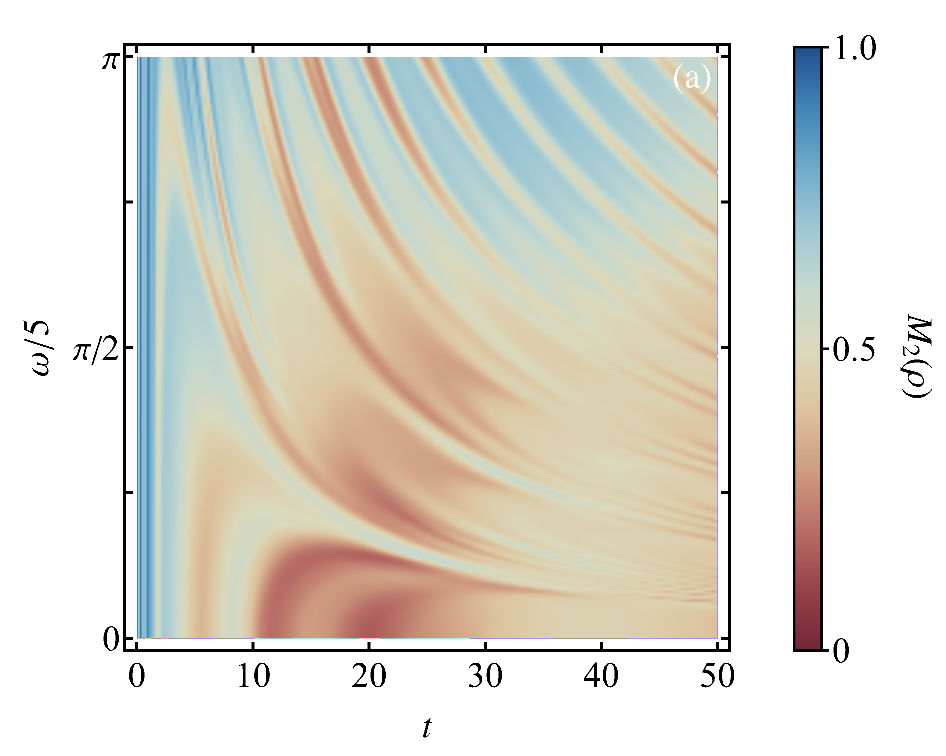
\includegraphics[width=\linewidth]{wolfram_plots/magic_plots/densityplot_cos1_magic.pdf}
    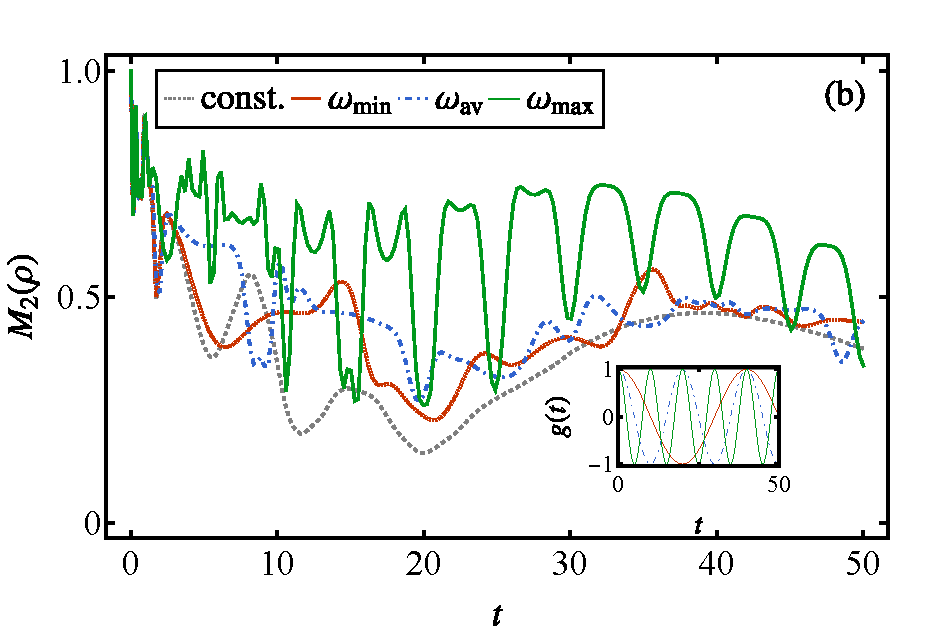
\includegraphics[width=\linewidth]{wolfram_plots/magic_plots/plottimeev_cos1_magic.pdf}
    \caption{
  Behavior of the normalized normalized $2$-Réniy entropy considering the initial state Eq. \eqref{eq:max_magic}, and the cosine modulation for the coupling, for different frequencies $\omega$ and fixing $\phi=0$. 
  In (a), we consider a density plot for the time evolution of $N(\rho)$ for the range of values  $\omega_{\text{min}}\leq\omega\leq\omega_{\text{max}}$, where $\omega_{\text{min}}=\pi/20$ and $\omega_{\text{max}}=\pi/5$.
   In (b), we present the time evolution for the constant coupling (dashed gray line), $\omega_{\text{min}}$ (dotted red line),
  $\omega_{\text{av}}=\omega_{\text{max}}/2$ (dot-dashed blue line) and
  $\omega_{\text{max}}$ (solid green line), with the time evolution of the coupling as an inset.
  }
    \label{fig:magic_cos1}
\end{figure}


\subsection{Entanglement}
\label{subsec:entanglement}
Entanglement is a distinctive form of quantum correlation associated with the non-separability of quantum states, and it constitutes a key resource for quantum technologies, enabling tasks in quantum computing, communication, and sensing that have no classical counterpart \cite{Horodecki2009, Browe2017, Sood2024}.

Quantifying entanglement is generally a nontrivial task, particularly for mixed states, which naturally arises in open quantum systems. To quantify the bipartite entanglement between the atom and the field, we employ the logarithmic negativity, defined as

\begin{equation}
    E_{\mathcal N}(\rho) = \log_2 \left\| \rho^{T_A} \right\|_1 ,
    \label{eq:entanglement}
\end{equation}
where $\rho^{T_A}$ denotes the partial transpose of the density operator with respect to subsystem $A$ and $\|\cdot\|_1$ is the trace norm. 
A nonzero value of $E_{\mathcal N}(\rho)$ signals the presence of entanglement, 
while $E_{\mathcal N}(\rho)=0$ indicates that no entanglement is detected by this measure \cite{Vidal2002}. 
\ts{Tenho a impressão de que você me falou que quando a negatividade é 0, não podemos afirmar nada? Ou isso vale só para a negatividade em si, e não para a escala log da transposta parcial da matriz densidade?}

To investigate this non-classicality, we consider the initial state
\begin{equation} \label{eq:entangled}
    |\psi(0)\rangle=\frac{1}{\sqrt{2}}\left(|e,\alpha\rangle +|g,-\alpha\rangle\right),
\end{equation}
which has a maximum $E_{\mathcal{N}}(\rho)=1$.
While the previous measures captured non-classicality within individual subsystems, entanglement fundamentally depends on the relations between subsystems. 
Consequently, we expect entanglement to be closely related to the interaction strength that couples them.

As in the case of coherence, we begin our analysis with the Gaussian coupling by varying $\zeta$ of the Gaussian envelope over the same interval while keeping the same values of $T=25$ and $\sigma=-1$. 
As shown in Fig.~\ref{fig:ent_gauss1}(a), the entanglement initially decays rapidly, given the  dissipative parameters employed and the fact that the subsystems are not interacting at the initial stage. 
However, as the coupling emerges (i.e., at the onset of the Gaussian tail), 
the entanglement increases and subsequently attenuates, 
mainly due to losses.
In the same figure, panel Fig.~\ref{fig:ent_gauss1}(b) shows a zoomed \ts{Esse zoomed se refere à escala log?} comparison between the selected values of $\zeta$ and the constant coupling, alongside the time dependence of the coupling strength in the inset. 
Note that, although the constant coupling is stronger at early times, which makes it dominant for approximately $t < 10$, the entanglement associated with the time-dependent coupling is comparatively heightened once the variable coupling becomes significant. 
In this regime, it reaches $E_{\mathcal{N}} \approx 0.5$ before decaying again, remaining higher than the constant-coupling case for most of the considered interval.

\begin{figure}[!h]
    \centering
    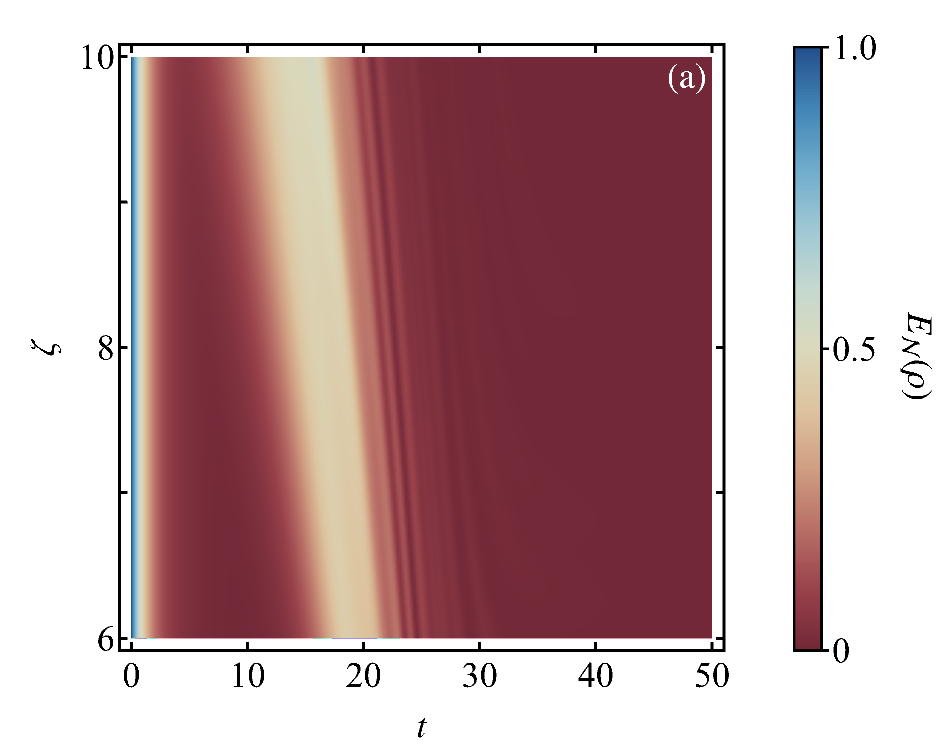
\includegraphics[width=\linewidth]{wolfram_plots/entanglement_plots/densityplot_gauss1_ent.pdf}
    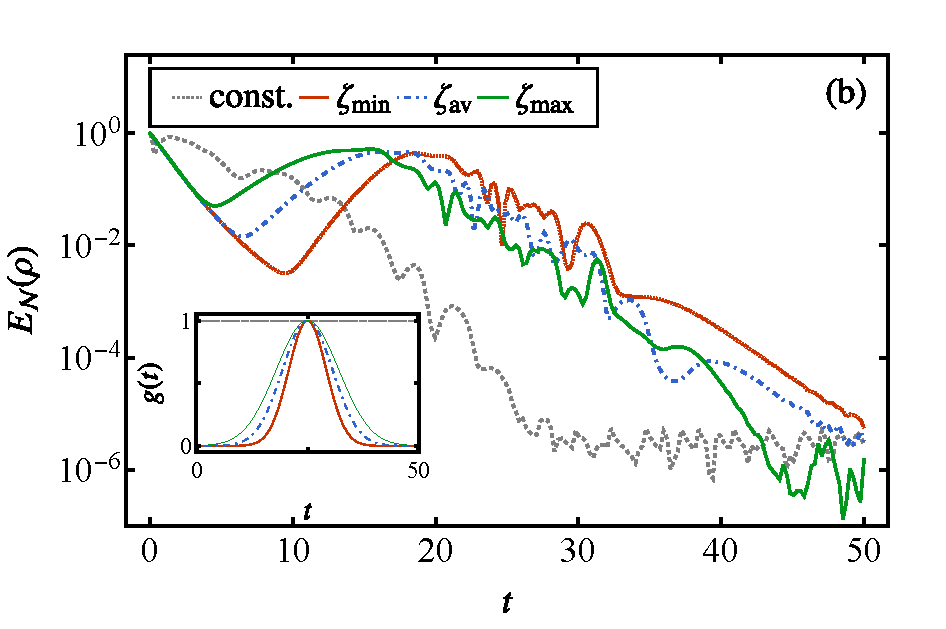
\includegraphics[width=\linewidth]{wolfram_plots/entanglement_plots/plottimeev_gauss1_ent.pdf}
    \caption{
    Behavior of the entanglement considering the initial state Eq. \eqref{eq:entangled}, and the gaussian modulation for the coupling, for different widths $\zeta$ of the gaussian envelope, fixing $T=25$ and $\sigma=-1$.
  In (a), we consider a density plot for the time evolution of $E_\mathcal{N}(t)$ for the range of values  $\zeta_{\text{min}} \leq \zeta \leq \zeta_{\text{max}}$, where $\zeta_{\text{min}}=6$ and $\zeta_{\text{max}}=10$.
   In (b), we present the time evolution for the constant coupling (dashed gray line), $\zeta_{\text{min}}$ (dotted red line),
  $\zeta_{\text{av}}=(\zeta_{\text{min}}+\zeta_{\text{max}})/2$ (dot-dashed blue line) and
  $\zeta_{\text{max}}$ (solid green line), with the time evolution of the coupling as an inset.
  }
    \label{fig:ent_gauss1}
\end{figure}

The same advantages can be observed when keeping the width constant while varying the position of the center of the Gaussian envelope, as shown in Fig. \ref{fig:ent_gauss3}. In this case, we observe that the earlier the peak of the coupling occurs, the larger the entanglement value reached after the onset of the dynamics. For the cases presented in Fig.~\ref{fig:ent_gauss3}(b), it can be seen that the rising of the coupling causes a growth in the entanglement. Additionally, the time-dependent coupling cases tends to sustain a larger of $E_\mathcal{N}(t)$ for a longer period compared to the constant coupling.

\begin{figure}
    \centering
    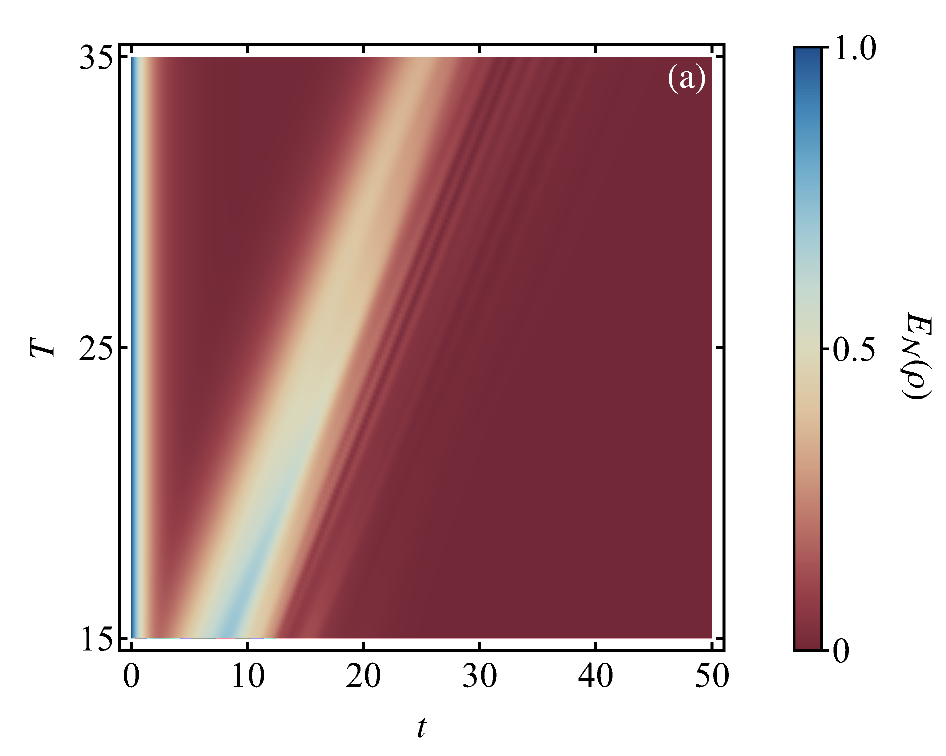
\includegraphics[width=\linewidth]{wolfram_plots/entanglement_plots/densityplot_gauss3_ent.pdf}
    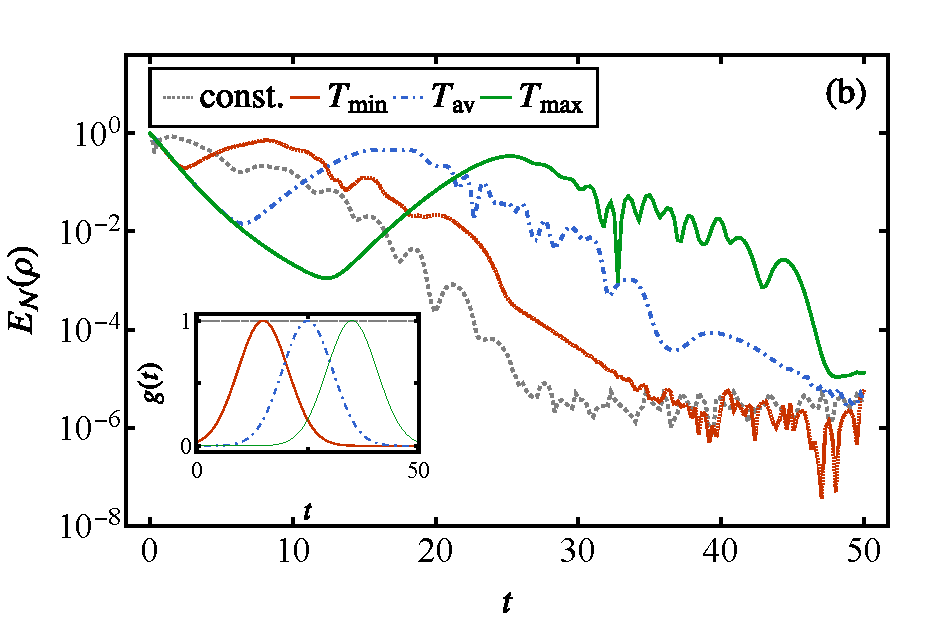
\includegraphics[width=\linewidth]{wolfram_plots/entanglement_plots/plottimeev_gauss3_ent.pdf}
    \caption{
  Behavior of the entanglement considering the initial state Eq. \eqref{eq:entangled}, and the gaussian modulation for the coupling, for different instants of peak $T$ of the gaussian envelope, fixing $\zeta=8$ and $\sigma=-1$.
  In (a), we consider a density plot for the time evolution of $E_\mathcal{N}(t)$ for the range of values  $T_{\text{min}}\leq T \leq T_{\text{max}}$, where $T_{\text{min}}=15$ and $T_{\text{max}}=35$.
   In (b), we present the time evolution for the constant coupling (dashed gray line), $T_{\text{min}}$ (dotted red line),
  $T_{\text{av}}=(T_{\text{min}}+T_{\text{max}})/2$ (dot-dashed blue line) and
  $T_{\text{max}}$ (solid green line), with the time evolution of the coupling as an inset.
  }
    \label{fig:ent_gauss3}
\end{figure}

Thus, this modulation may substantially amplify maintenance of entanglement in the system.
Although this advantage is not observed at the initial stages, since the systems are not yet effectively interacting, the subsequent dynamics favors a stronger and more persistent entanglement.

For the cosine coupling, displayed in Fig. \ref{fig:ent_cos6}, we choose initial conditions such that $g(0) = 1$, establishing a different starting point for the dynamics, with atom and cavity interacting at the outset.
In panel (a), the influence of the coupling is clearly visible through its undulatory pattern, which induces oscillations in the entanglement until it eventually reaches negligible values. 
In Fig.~\ref{fig:ent_cos6}(b), we observe that although these oscillations may reach smaller values at certain times, for different values of $\omega$ they remain significantly larger over several time intervals when compared to the constant coupling case, as quantified by $E_{\mathcal{N}}(\rho)$.
This result demonstrates that advantages of employing a time-dependent coupling can also be obtained when the initial coupling is maximal, in contrast to the previously discussed Gaussian coupling scenario.

\begin{figure}
    \centering
    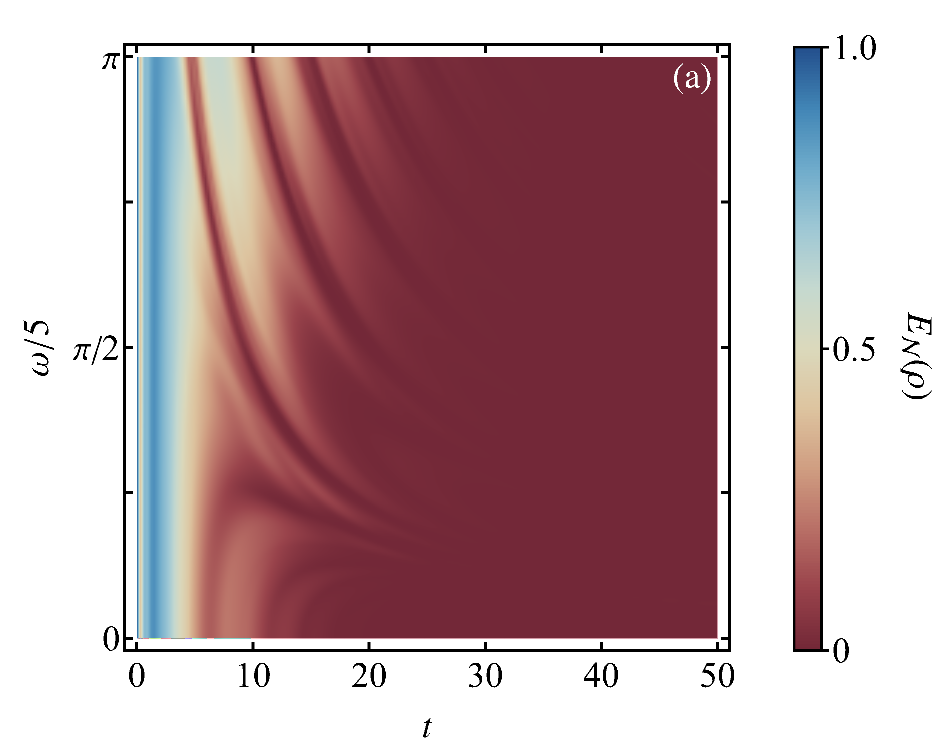
\includegraphics[width=\linewidth]{wolfram_plots/entanglement_plots/densityplot_cos6_ent.pdf}
    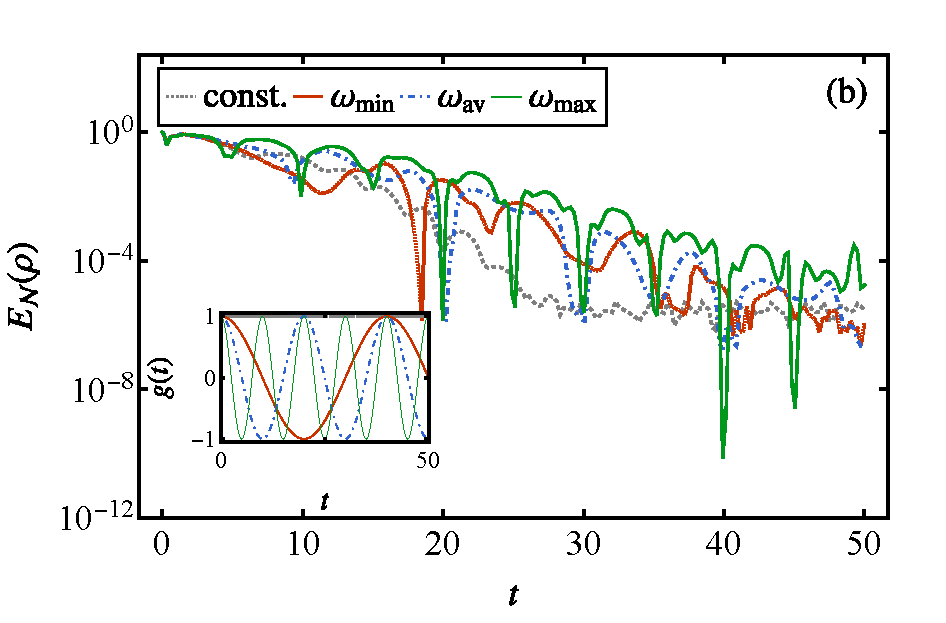
\includegraphics[width=\linewidth]{wolfram_plots/entanglement_plots/plottimeev_cos6_ent.pdf}
    \caption{
  Behavior of the entanglement considering the initial state Eq. \eqref{eq:entangled}, and the cosine modulation for the coupling, for different frequencies $\omega$ and fixing $\phi=0$. 
  In (a), we consider a density plot for the time evolution of $E_\mathcal{N}(t)$ for the range of values  $\omega_{\text{min}}\leq\omega\leq\omega_{\text{max}}$, where $\omega_{\text{min}}=\pi/20$ and $\omega_{\text{max}}=\pi/5$.
   In (b), we present the time evolution for the constant coupling (dashed gray line), $\omega_{\text{min}}$ (dotted red line),
  $\omega_{\text{av}}=(\omega_{\text{min}}+\omega_{\text{max}})/2=8$ (dot-dashed blue line) and
  $\omega_{\text{max}}$ (solid green line), with the time evolution of the coupling as an inset.
  }
    \label{fig:ent_cos6}
\end{figure}



%---------------------------------%
\section{Conclusions}
\label{sec:Conc}

%----------------------------------------------------------------------%
\section*{Acknowledgements}

T. T. T. would like to acknowledge financial support from Coordenação de Aperfeiçoamento
de Pessoal de N\'{i}vel Superior (CAPES, Finance Code 001). 

%----------------------------------------------------------------------%

\bibliographystyle{apsrev4-2}
\bibliography{refs.bib}

\end{document} 